% Informe Final de Año de Prácticas
% Cesar Alejandro Barillas Segura
% ECFM-USAC
%
% Este documento unifica el anteproyecto (mayo 2024) con los resultados
% experimentales y numéricos obtenidos durante el año de prácticas.

\documentclass[titlepage,11pt]{article}

%%% PAQUETES
\usepackage[spanish,es-nodecimaldot]{babel}%
\usepackage[utf8]{inputenc}%
\usepackage{graphicx}%
\usepackage{latexsym}%
\usepackage{amsfonts, amsmath, amssymb}%
\usepackage{physics}
\usepackage{float}
\usepackage[amssymb]{SIunits}%
% SIunits no define \num ni \SI (son de siunitx); se añaden como atajos
% para que el texto quede uniforme sin cambiar de paquete de unidades.
\providecommand{\num}[1]{\ensuremath{#1}}
\providecommand{\SI}[2]{#1\,#2}
\providecommand{\percent}{\char37\relax}
\usepackage[letterpaper, bottom=25mm, top=25mm]{geometry}
\usepackage[table]{xcolor}
\usepackage{longtable}
\usepackage{array}
\usepackage{booktabs}
\usepackage{multirow}
\usepackage{csquotes}

\usepackage[bookmarksnumbered, breaklinks={true},%
pdfauthor={Alejandro Barillas (alejandroecfm@gmail.com)},%
pdftitle={Redes neuronales de aprendizaje automático para la Inferencia de modelos físicos},%
pdfsubject={F\'isica Computacional},%
pdfkeywords={Physical Systems \& Artificial neural networks \& Machine learning}]{hyperref}


\begin{document}
% % % % % % % % % % % % % % % % % % % % % % % % % % % % % % % % % % %
\begin{titlepage}
  \pagestyle{empty}
  \pdfbookmark[0]{Title}{title}
  \begin{center}
    \begin{minipage}{\textwidth}
      \begin{minipage}[c]{0.45\textwidth}
        \centering 
\includegraphics[width=.8\textwidth]{usacAzul}
      \end{minipage}%
      \hfill
      \begin{minipage}[c]{0.45\textwidth}
        \vspace{-1em}
\includegraphics[width=.85\textwidth]{ecfmAzul}
      \end{minipage}
    \end{minipage}

    \vspace{2em}
    \begin{minipage}[t]{.95\textwidth}
      \centering\large
      \textsc{Universidad de San Carlos de Guatemala\\
        Escuela de Ciencias Físicas y Matemáticas}
    \end{minipage}

    \vspace{1em}\noindent\rule{\textwidth}{1px}\vfill
    \begin{minipage}[t]{.95\textwidth}
      \centering\Huge
      \textsc{Redes Neuronales de Aprendizaje Automático para la Inferencia de Modelos Físicos}
    \end{minipage}

    \vfill
    \begin{minipage}[t]{.75\textwidth}
      \centering
      Informe Final de Año de Prácticas elaborado por\\%
      \textbf{Cesar Alejandro Barillas Segura}\\
      presentado ante el Departamento de Física
    \end{minipage}

    \vfill
    \begin{minipage}[t]{.95\textwidth}
      \centering
      Supervisado por \\%
      Dr. Giovanni Ramírez García (ECFM-USAC)
    \end{minipage}

    \vfill\noindent\rule{\textwidth}{1px}
    \begin{minipage}[t]{.95\textwidth}
      \centering
      Guatemala, \today
    \end{minipage}
  \end{center}
\end{titlepage}
% % % % % % % % % % % % % % % % % % % % % % % % % % % % % % % % % % %

\pagestyle{empty}
\setcounter{page}{0}

% % % % % % % % % % % % % % % % % % % % % % % % % % % % % % % % % % %
\section*{Resumen}
\addcontentsline{toc}{section}{Resumen}

Se estudió si una red neuronal entrenada con datos experimentales de caída
libre es capaz de inferir el modelo físico que los genera, es decir, si de la
red entrenada puede recuperarse la aceleración de la gravedad~$g$. Se grabaron
609 clips de video a \unit{60}{\hertz} de un cuerpo en caída libre, se
digitalizaron sus trayectorias con \emph{Tracker} y se obtuvieron
\num{20\,210} pares $(t,y)$ útiles repartidos en 606 clips. Con esos datos se
entrenaron tres arquitecturas en PyTorch: una red mínima $1\to2\to1$ que
recibe únicamente el tiempo, una red $3\to4\to1$ que recibe tiempo, velocidad
y aceleración verticales, y una red profunda con activaciones $\tanh$
($1\to32\to32\to1$). El desempeño se midió con RMSE y MAE sobre la posición, y
la inferencia del modelo físico se evaluó ajustando una parábola
$y=c_0+c_1t+c_2t^2$ a las predicciones y comparando $g=2c_2$ con el valor
obtenido de los datos experimentales.

Las tres redes alcanzan errores de posición muy parecidos
(RMSE entre \num{0.507} y \num{0.514}~\meter), pero ese valor apenas mejora al
de un predictor trivial que devuelve siempre la posición media
(RMSE~$=\num{0.619}$~\meter), lo que corresponde a un coeficiente de
determinación $R^2\approx\num{0.31}$. Al estimar $g$ \emph{clip por clip} ---
que es el único nivel en el que la cantidad tiene sentido físico --- los datos
experimentales dan $g=\num{-9.00}\pm\num{2.36}$~\meter\per\second\squared{}
(mediana \num{-9.38}), consistente con el valor esperado, mientras que las
redes devuelven $\num{0.17}$, $\num{-3.25}$ y
$\num{-3.60}$~\meter\per\second\squared{} respectivamente. Con el planteamiento
inicial, por tanto, \textbf{las redes no infieren el modelo físico}: al agrupar
606 trayectorias con distinta altura inicial y distinto origen temporal bajo un
único mapeo $y=f(t)$, el problema deja de ser identificable y la mejor solución
posible es la media condicional de los datos, que es justamente lo que las
redes aprenden. El fallo es de planteamiento, no de capacidad.

A partir de ese diagnóstico se rehízo el experimento refiriendo cada clip a su
propio origen, con entradas $(\tau,v_0)$ y salida $\Delta y$, particionando por
clip completo, con cinco semillas y tres líneas base clásicas de referencia.
Con las \emph{mismas} arquitecturas y los \emph{mismos} datos, la red $\tanh$
profunda pasa de $R^2=\num{0.33}$ a $R^2=\num{0.93}$ y recupera
$g=\num{-9.46}\pm\num{0.33}~\meter\per\second\squared$, a un
\SI{0.2}{\percent} del valor que el método clásico extrae de esos mismos datos
($\num{-9.48}~\meter\per\second\squared$), además de superar en un
\SI{30}{\percent} al modelo analítico de MRUV con una única $g$ ajustada. El
supuesto del anteproyecto queda así verificado, y el informe documenta tanto el
diagnóstico del fallo inicial como la reformulación que lo corrige.

\newpage
\pagestyle{plain}
\tableofcontents
\newpage


% % % % % % % % % % % % % % % % % % % % % % % % % % % % % % % % % % %
\section{Descripción general de la Institución}
\label{sec:institucion}
La Universidad de San Carlos de Guatemala (USAC) es la institución de
educación superior estatal, autónoma, con cultura democrática, con enfoque
multi e intercultural, vinculada y comprometida con el desarrollo científico,
social, humanista y ambiental, con una gestión actualizada, dinámica, efectiva
y con recursos óptimamente utilizados para alcanzar sus fines y objetivos. Es
la universidad más antigua de Guatemala, habiendo sido fundada el 31 de enero
de 1676. El campus central se encuentra ubicado en el Departamento de
Guatemala, Ciudad Universitaria 11 Avenida, Zona 12. Su lema es \emph{Id y
  enseñad a todos}.

La Escuela de Ciencias Físicas y Matemáticas (ECFM) es una escuela no
facultativa formada en el año 2009 en el evento CONVERGENCIA. Actualmente, la
escuela cuenta con la carrera de Licenciatura en Física Aplicada y
Licenciatura en Matemática Aplicada. La escuela cuenta también con un
Instituto dedicado a la investigación de las ciencias físicas y matemáticas
(IFIM) el cual ha presentado diversas investigaciones y publicado una variedad
de artículos relacionados con la divulgación del conocimiento de las ciencias.

El IFIM es la unidad de la ECFM que promueve y realiza estudios avanzados en
áreas científicas fundamentales y aplicadas de las ciencias físicas y
matemáticas.  Las áreas y líneas de investigación del Instituto son
\begin{enumerate}
\item Física de altas energías, cosmología y astrofísica: Física de
  partículas, Astrofísica de rayos gamma.
\item Ciencias no lineales y sistemas complejos: Materia condensada, Modelos
  numéricos del clima, Modelos matemáticos en ciencias de la salud.
\item Geofísica: Geodesia aplicada a la tectónica.
\item Física experimental: Detección de partículas e instrumentación
  electrónica, Redes de sensores.
\item Física de radiaciones: Control de calidad en radioterapia.
\end{enumerate}

Además, el Instituto realiza actividades de difusión y divulgación, Seminarios
científicos, Conferencias de divulgación científica y también Talleres y
cursos cortos.


% % % % % % % % % % % % % % % % % % % % % % % % % % % % % % % % % % %
\section{Descripción del grupo de trabajo}
\label{sec:grupo}
La Física de Materia Condensada es un área muy amplia e interesante. Mediante
el estudio de las propiedades fundamentales de la materia se pueden observar
fenómenos interesantes que permiten el desarrollo de nuevas tecnologías. En
años recientes la relación entre éstos fenómenos a nivel subatómico y las
propiedades generales de los materiales ha permitido el desarrollo de
materiales con nuevas propiedades o materiales de diseño.

Por otro lado, uno de los desarrollos más excitantes de la Física en los
últimos años es la convergencia entre la Física de la Materia Condensada y las
áreas de Información Cuántica y Computación Cuántica, lo que ha permitido un
avance acelerado en ambos campos llevando de la mano a la teoría y al
experimento. El principal motivo de esta convergencia es el estudio de los
sistemas cuánticos de muchos cuerpos donde es indispensable entender el
entrelazamiento cuántico que resulta ser el recurso principal para la teoría
de información cuántica.

El Grupo de investigación se enfoca en las áreas de la física de la materia
condensada, incluyendo varios grupos de estudio aplicados a mecánica
estadística, mecánica cuántica, óptica, nanociencia, información cuántica,
computación cuántica, etc.


% % % % % % % % % % % % % % % % % % % % % % % % % % % % % % % % % % %
\section{Introducción}
\label{sec:introduccion}
En este proyecto se aprendió a programar, entrenar y estudiar las
características internas de una red neuronal dedicada a la identificación de
modelos físicos. El caso de estudio es la caída libre de un cuerpo, descrita
por el movimiento rectilíneo uniformemente variado (MRUV) que se detalla en la
sección~\ref{subsec:mru}. Los conocimientos matemáticos necesarios para
construir y entrenar la red --- suma ponderada, mínimos cuadrados, derivadas
parciales y regla de la cadena --- se resumen en la
sección~\ref{subsec:mat}. La parte técnica y descriptiva de las redes
neuronales, su arquitectura, sus funciones de activación y sus funciones de
coste, se trata en la sección~\ref{subsec:redneuronal}, y el mecanismo de
aprendizaje en la sección~\ref{subsec:ML}. La implementación se realizó en
PyTorch (sección~\ref{subsec:ts}).

La pregunta que organiza todo el trabajo no es si una red puede ajustar una
curva --- eso se sabe desde hace décadas --- sino si de una red ya entrenada
puede \emph{extraerse} el modelo físico subyacente. Concretamente: si se
entrena una red con trayectorias reales de caída libre y después se ajusta una
parábola a sus predicciones, ¿aparece el valor correcto de~$g$? Ese es el
criterio de éxito que se adoptó, y responderlo requiere tanto un montaje
experimental que produzca datos suficientes (sección~\ref{sec:datos}) como un
protocolo de evaluación que sea válido (sección~\ref{sec:protocolo}).

Conviene adelantar el desenlace, porque condiciona la lectura del resto del
documento. El trabajo tiene dos partes. En la primera, con el planteamiento tal
como se concibió en el anteproyecto, la respuesta es \emph{negativa}: las redes
no recuperan~$g$. La razón no está en su capacidad sino en cómo se formuló el
problema de aprendizaje, y la sección~\ref{sec:resultados} presenta la evidencia
junto con el diagnóstico (sección~\ref{subsec:identificabilidad}).

En la segunda parte se corrige ese planteamiento y se repite el experimento con
las mismas arquitecturas y los mismos datos. La respuesta pasa a ser
\emph{afirmativa}: la red recupera la gravedad con una discrepancia del
\SI{0.2}{\percent} respecto de lo que el método clásico obtiene de esos mismos
datos (sección~\ref{sec:v2}). El supuesto del anteproyecto queda verificado, y
el camino que llevó hasta ahí --- un resultado negativo bien caracterizado que
indica exactamente qué cambiar --- es en sí mismo el aprendizaje central del
proyecto.

\subsection{Movimiento rectilíneo uniformemente variado}
\label{subsec:mru}

Un cuerpo que se mueve en línea recta con aceleración constante~$a$ describe
la posición
\begin{equation}
  y(t) = y_0 + v_0\,t + \frac{1}{2}a\,t^2,
  \label{eq:mruv}
\end{equation}
donde $y_0$ es la posición en $t=0$ y $v_0$ la velocidad inicial. En caída
libre, despreciando el arrastre del aire, la aceleración es la de la gravedad,
$a=g$. Con el eje $y$ orientado hacia arriba --- que es la convención que usa
\emph{Tracker} y la que se mantiene en todo este informe ---
$g\approx\num{-9.81}~\meter\per\second\squared$, y tanto $y$ como $v_0$ pueden
ser negativos.

La ecuación~\eqref{eq:mruv} es el \enquote{marco teórico} cuya recuperación se
busca. Tres observaciones sobre su estructura resultan decisivas más adelante:

\begin{enumerate}
\item $g$ aparece únicamente en el coeficiente cuadrático. Si se ajusta
  $y=c_0+c_1t+c_2t^2$ a una trayectoria, entonces $g=2c_2$, y ese es el
  estimador que se usa en todo el trabajo.
\item Los tres coeficientes son independientes: $y_0$ y $v_0$ son propios de
  cada lanzamiento, mientras que $g$ es común a todos. Una trayectoria queda
  determinada por la terna $(y_0,v_0,g)$, no por $g$ sola.
\item Por lo tanto, $t$ \emph{no} determina $y$. Dos lanzamientos distintos
  con la misma $t$ tienen posiciones distintas si difieren en $y_0$ o $v_0$.
  Esta observación, aparentemente trivial, es la que explica los resultados de
  la sección~\ref{sec:resultados}.
\end{enumerate}

\subsection{Herramientas Matemáticas}
\label{subsec:mat}

\subsubsection{Suma ponderada}
Una neurona artificial toma entradas $(x_1,x_2,\ldots,x_n)$ y pesos
$(w_1,w_2,\ldots,w_n)$. La suma ponderada se calcula multiplicando cada
entrada por su peso correspondiente y sumando los resultados,
\begin{equation}
  z = w_1x_1 + w_2x_2 + \cdots + w_nx_n + b,
\end{equation}
donde $b$ es el sesgo, un valor constante. La suma ponderada pesa las entradas
según su importancia relativa; esos pesos se adaptan durante el
entrenamiento~\cite{triola_2018_estadstica}.

\subsubsection{Mínimos cuadrados y ajuste polinómico}
\label{subsubsec:minimoscuadrados}
Dada una colección de datos, la recta de regresión es la que mejor se ajusta a
ellos bajo el criterio de mínimos cuadrados, $\hat y = b_0+b_1x$. El mismo
criterio se generaliza a cualquier modelo lineal en los parámetros, y en
particular a la parábola que interesa aquí. Dados $N$ pares $(t_i,y_i)$ se
construye la matriz de diseño
\begin{equation}
  \mathbf{T} =
  \begin{pmatrix}
    1 & t_1 & t_1^2\\
    1 & t_2 & t_2^2\\
    \vdots & \vdots & \vdots\\
    1 & t_N & t_N^2
  \end{pmatrix},
  \qquad
  \mathbf{c} = (c_0,c_1,c_2)^{\mathsf T},
\end{equation}
y se busca el $\mathbf{c}$ que minimiza $\norm{\mathbf{T}\mathbf{c}-\mathbf{y}}^2$,
cuya solución es $\mathbf{c}=(\mathbf{T}^{\mathsf T}\mathbf{T})^{-1}\mathbf{T}^{\mathsf T}\mathbf{y}$.
Comparando con~\eqref{eq:mruv} se identifica $c_0=y_0$, $c_1=v_0$ y
$g=2c_2$. Este ajuste es la herramienta central del trabajo: se aplica tanto a
los datos experimentales como a las predicciones de cada red, y la comparación
entre ambos valores de $g$ es el criterio con el que se juzga si la red capturó
la física~\cite{triola_2018_estadstica}.

Es importante notar una propiedad de este estimador que se explotará en la
discusión: el ajuste solo tiene significado físico si todos los puntos
$(t_i,y_i)$ que entran en él pertenecen a \emph{una misma trayectoria}. Si se
mezclan trayectorias con distinto $y_0$, distinto $v_0$ o distinto origen
temporal, el $c_2$ resultante no es $g/2$ sino un número sin interpretación.

\subsubsection{Coeficiente de determinación}
Para juzgar si un modelo aporta información sobre la simple media de los datos
se usa
\begin{equation}
  R^2 = 1 - \frac{\sum_i (y_i-\hat y_i)^2}{\sum_i (y_i-\bar y)^2},
  \label{eq:r2}
\end{equation}
donde $\bar y$ es la media muestral. $R^2=1$ corresponde a predicción perfecta
y $R^2=0$ al desempeño de un modelo que devuelve siempre $\bar y$. Esta métrica
resulta indispensable porque un RMSE \enquote{pequeño} solo significa algo al
compararlo con la dispersión propia de los datos.

\subsubsection{Derivadas parciales}
Las derivadas parciales proporcionan información sobre cómo una función cambia
respecto de cada una de sus variables independientes. Para
$z=f(x_1,x_2,\ldots,x_n)$ se define
\begin{equation}
  \pdv{z}{a}=\lim_{\Delta a\to0}
  \frac{f(x_1,\ldots,a+\Delta a,\ldots,x_n)-f(x_1,\ldots,x_n)}{\Delta a},
\end{equation}
donde $a$ es cualquiera de las variables de la función~\cite{zill_1985_clculo}.
En una red neuronal, las derivadas parciales de la función de coste respecto de
cada peso son exactamente lo que el algoritmo de entrenamiento necesita para
saber en qué dirección modificar ese peso.

\subsubsection{Regla de la cadena}
Si $z=f(u_1,u_2,\ldots,u_n)$ y cada $u_i$ es función de $x_1,x_2,\ldots,x_k$,
entonces~\cite{zill_1985_clculo}
\begin{equation}
  \pdv{z}{x_i}=\pdv{z}{u_1}\pdv{u_1}{x_i}+\pdv{z}{u_2}\pdv{u_2}{x_i}
  +\cdots+\pdv{z}{u_n}\pdv{u_n}{x_i},
  \label{eq:cadena}
\end{equation}
donde $i$ toma cualquier valor entero de 1 a $k$. Como una red neuronal es una
composición de funciones --- cada capa aplicada al resultado de la anterior ---
la ecuación~\eqref{eq:cadena} es literalmente el mecanismo que permite
propagar el error desde la salida hasta la primera capa, y por eso reaparece en
la sección~\ref{subsec:ML}.

\subsubsection{Normalización de los datos}
\label{subsubsec:zscore}
Antes de entrenar conviene llevar entradas y salidas a una escala común. La
normalización $z$ transforma cada variable según
\begin{equation}
  \tilde x = \frac{x-\mu_x}{\sigma_x},
  \label{eq:zscore}
\end{equation}
con $\mu_x$ y $\sigma_x$ la media y la desviación estándar muestrales. Esto
evita que variables con rangos muy distintos --- aquí, tiempos del orden de
$10^{-1}$~\second\ y posiciones del orden de $1$~\meter\ --- produzcan
gradientes de magnitudes desbalanceadas. Las predicciones se
desnormalizan con la transformación inversa antes de calcular cualquier
métrica física, de modo que todos los errores reportados en este informe están
en metros.

\subsection{Red Neuronal}
\label{subsec:redneuronal}

\subsubsection{Neurona}
Una red neuronal es un conjunto interconectado de nodos llamados neuronas
artificiales. Estas neuronas están organizadas en capas y se comunican entre sí
mediante conexiones ponderadas. Cada neurona toma la información de entrada,
hace una suma ponderada, le aplica una función de activación y transmite el
resultado a la siguiente neurona o, en su defecto, a la
salida~\cite{antonio_2023_introduccin,ibm_qu,santana_2018_1,santana_2018_2,santana_2018_3,santana_2018_3_5}.

\subsubsection{Capas}
Hay diferentes tipos de capas neuronales:
\begin{itemize}
\item \textbf{Capa de entrada:} recibe los valores de entrada de la red.
\item \textbf{Capas ocultas:} procesan la información de manera intermedia.
\item \textbf{Capa de salida:} entrega los datos de salida de la red.
\end{itemize}
Cada neurona artificial se conecta a otras y tiene un peso y un umbral
asociados. Si la salida de una neurona está por encima del umbral, se activa y
envía datos a la siguiente capa; de lo contrario no propaga
información~\cite{antonio_2023_introduccin,ibm_qu}.

El número de neuronas ocultas fija la \emph{capacidad expresiva} de la red: una
red con dos neuronas ocultas y activación ReLU solo puede representar funciones
lineales a trozos con a lo sumo dos quiebres, mientras que dos capas de 32
neuronas $\tanh$ pueden aproximar cualquier función continua sobre un intervalo
acotado con la precisión que se desee. Este contraste es deliberado en el
diseño experimental de la sección~\ref{subsec:arquitecturas}.

\subsubsection{Función de activación}
La función de activación determina la salida de una neurona a partir de su suma
ponderada. Su papel es introducir no linealidad: sin ella, una red de cualquier
profundidad colapsa a una única transformación
lineal~\cite{wikipediacontributors_2018_activation}. Para un valor $x$ igual a
la suma ponderada de entradas y pesos, las funciones más comunes son:

\begin{enumerate}
\item \textbf{Función sigmoide:} lleva los valores al intervalo $(0,1)$. Se usa
  sobre todo cuando se necesita predecir probabilidades, como en clasificación
  binaria. Su ecuación es
  \begin{equation}
    f(x)=\frac{1}{1+e^{-x}}.
  \end{equation}

  \begin{figure}[H]
    \centering
    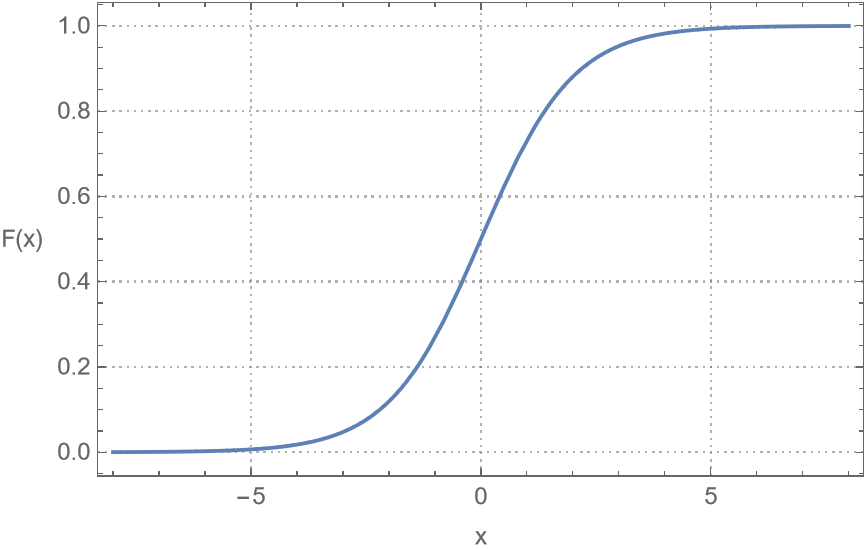
\includegraphics[width=0.4\linewidth]{sigmoide}
    \caption{Gráfica de la función sigmoide. Fuente: elaboración propia.}
    \label{fig:sigmoide}
  \end{figure}

\item \textbf{Tangente hiperbólica ($\tanh$):} su rango es $(-1,1)$. Es similar
  a la sigmoide pero centrada en el origen, lo que suele mejorar la
  convergencia. Su ecuación es
  \begin{equation}
    f(x)=\frac{e^{x}-e^{-x}}{e^{x}+e^{-x}}.
  \end{equation}

  \begin{figure}[H]
    \centering
    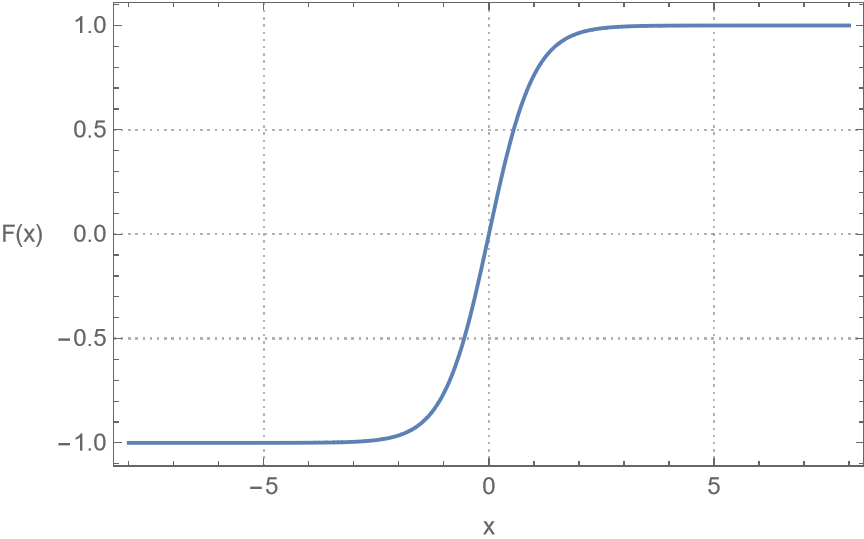
\includegraphics[width=0.4\linewidth]{tanh}
    \caption{Gráfica de la función tangente hiperbólica. Fuente: elaboración
      propia.}
    \label{fig:tanh}
  \end{figure}

\item \textbf{Rectificadora lineal (ReLU):} devuelve 0 para valores negativos y
  el valor original para valores positivos,
  \begin{equation}
    f(x)=\max(0,x).
  \end{equation}

  \begin{figure}[H]
    \centering
    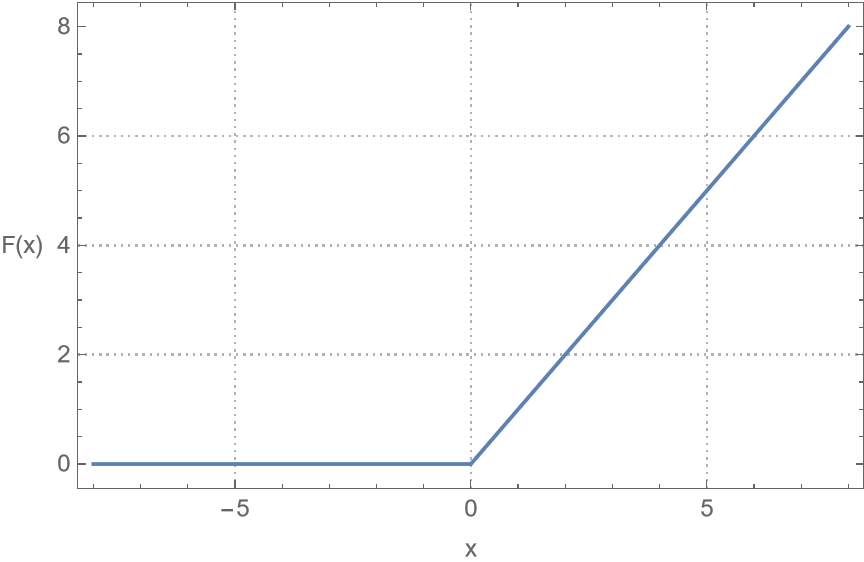
\includegraphics[width=0.4\linewidth]{relu}
    \caption{Gráfica de la función ReLU. Fuente: elaboración propia.}
    \label{fig:relu}
  \end{figure}

  La ReLU es barata de evaluar y su derivada no se satura para $x>0$, pero
  tiene un modo de falla conocido: si durante el entrenamiento el argumento de
  una neurona se vuelve negativo para todos los datos, su gradiente es cero de
  forma permanente y la neurona deja de aprender. Este fenómeno, llamado
  \emph{ReLU muerta}, es más probable cuanto menos neuronas tenga la capa, y se
  invocará en la sección~\ref{subsec:epocas} para explicar el comportamiento de
  la red $1\to2\to1$.
\end{enumerate}

\subsubsection{Función de coste}
\label{subsubsec:coste}
La función de coste mide el error entre el valor estimado y el valor real
durante el entrenamiento. Su minimización es el objetivo de todo el
proceso~\cite{antonio_2023_introduccin,ibm_qu}. Con $\hat y_i$ la predicción,
$y_i$ el valor real y $n$ el número de muestras:

\begin{enumerate}
\item \textbf{Error cuadrático medio (MSE):} es la función que se minimiza
  durante el entrenamiento,
  \begin{equation}
    \mathrm{MSE}=\frac{1}{n}\sum_{i=1}^{n}(\hat y_i-y_i)^2.
  \end{equation}

\item \textbf{Raíz del error cuadrático medio (RMSE):} es la raíz del anterior,
  \begin{equation}
    \mathrm{RMSE}=\sqrt{\frac{1}{n}\sum_{i=1}^{n}(\hat y_i-y_i)^2},
  \end{equation}
  con la ventaja de estar en las mismas unidades que la variable predicha ---
  metros, en este trabajo. Penaliza fuertemente los errores grandes.

\item \textbf{Error absoluto medio (MAE):} promedia los valores absolutos de
  los errores,
  \begin{equation}
    \mathrm{MAE}=\frac{1}{n}\sum_{i=1}^{n}\abs{\hat y_i-y_i}.
  \end{equation}
  Es más fácil de interpretar que el RMSE y menos sensible a valores atípicos.
\end{enumerate}

Un punto que conviene subrayar, porque se vuelve central en el análisis: MSE,
RMSE y MAE son medidas \emph{relativas}. Un RMSE de \num{0.5}~\meter\ es
excelente si los datos varían en decenas de metros y es pésimo si varían en
centímetros. Por eso todo RMSE reportado aquí se acompaña del RMSE del
predictor constante $\hat y=\bar y$, cuyo valor es exactamente la desviación
estándar de los datos, y del $R^2$ de la ecuación~\eqref{eq:r2}.

Además, existen optimizadores que usan estas funciones de coste para ajustar
los pesos:
\begin{itemize}
\item \textbf{Descenso estocástico del gradiente (SGD):} actualiza los pesos en
  la dirección opuesta al gradiente estimado sobre un subconjunto (lote) de los
  datos, $w \leftarrow w - \eta\,\partial C/\partial w$, con $\eta$ la tasa de
  aprendizaje.
\item \textbf{Adam:} adapta la tasa de aprendizaje de cada parámetro usando
  estimaciones del primer y segundo momento del gradiente. Es el optimizador
  empleado en todos los entrenamientos de este trabajo, con
  $\eta=10^{-3}$.
\end{itemize}

\subsection{Aprendizaje automático}
\label{subsec:ML}

\subsubsection{Backpropagation}
El \emph{backpropagation}, o propagación hacia atrás de errores, es el
algoritmo fundamental del aprendizaje supervisado en redes neuronales. Su
objetivo es ajustar los pesos para minimizar el error entre las predicciones y
los valores reales, y consiste en aplicar la regla de la
cadena~\eqref{eq:cadena} desde la salida hacia la entrada: se calcula el error
en la capa de salida, se propaga hacia atrás capa por capa multiplicando por
las derivadas locales, y con las derivadas parciales resultantes
$\partial C/\partial w$ el optimizador actualiza cada peso. El ciclo completo
sobre todo el conjunto de entrenamiento es una \emph{época}.

\subsubsection{Sobreajuste y validación}
\label{subsubsec:sobreajuste}
Entrenar durante muchas épocas puede llevar a que la red memorice
particularidades del conjunto de entrenamiento en lugar de aprender la
regularidad subyacente. Para detectarlo se separan los datos en un conjunto de
entrenamiento y uno de validación, y se vigila que el error de validación no
empiece a crecer mientras el de entrenamiento sigue bajando.

La forma en que se hace esa separación importa tanto como el hecho de hacerla.
Si los datos provienen de experimentos repetidos, repartir los puntos
individuales al azar hace que puntos de una misma trayectoria caigan a ambos
lados de la partición; entonces el conjunto de validación no mide capacidad de
generalización a un experimento nuevo, sino solo de interpolación dentro de
experimentos ya vistos. La alternativa correcta es particionar por experimento
completo (validación \emph{leave-one-clip-out}). Este trabajo empleó la
partición aleatoria por puntos, y en la sección~\ref{sec:limitaciones} se
discuten sus consecuencias.

\subsubsection{Identificabilidad del modelo}
\label{subsubsec:identificabilidad-teoria}
Existe una condición previa a cualquier consideración de arquitectura o de
entrenamiento, y es que el problema planteado tenga solución. Si se busca una
función $f$ tal que $y\approx f(x)$ y en los datos existen pares $(x,y_a)$ y
$(x,y_b)$ con $y_a\neq y_b$, ninguna función puede reproducir ambos: el
problema es \emph{no identificable} a partir de $x$.

En ese caso la teoría de la regresión da una respuesta precisa. El minimizador
del error cuadrático esperado es la media condicional,
\begin{equation}
  f^{\star}(x)=\mathbb{E}[\,y\mid x\,],
  \label{eq:mediacondicional}
\end{equation}
y el error residual mínimo alcanzable es la varianza condicional
$\mathbb{E}[\operatorname{Var}(y\mid x)]$, que no puede reducirse por más
capacidad o más épocas que se le den al modelo. Una red suficientemente
expresiva entrenada con MSE converge a~\eqref{eq:mediacondicional}, no a la ley
física que generó los datos. Distinguir un fallo de este tipo de un fallo de
capacidad o de entrenamiento es esencial para interpretar correctamente los
resultados de la sección~\ref{sec:resultados}.

\subsection{PyTorch}
\label{subsec:ts}
El anteproyecto contemplaba usar TensorFlow~\cite{TensorFlow}, la plataforma de
aprendizaje automático desarrollada por Google y liberada en 2015. Durante la
implementación se migró a \textbf{PyTorch}, biblioteca de código abierto
mantenida por Meta AI, por dos razones prácticas: su modo de ejecución
inmediata (\emph{eager}) permite inspeccionar tensores y gradientes con un
depurador convencional, lo que resultó decisivo para un proyecto cuyo objetivo
es \emph{estudiar} el interior de la red y no solo entrenarla; y su API de
módulos (\texttt{torch.nn}) expresa arquitecturas pequeñas y no estándar con
menos código intermedio. Ambas bibliotecas implementan diferenciación
automática sobre grafos de cómputo y son equivalentes para los fines de este
trabajo. Los conceptos descritos en las secciones anteriores --- capas
lineales, activaciones, función de coste, optimizador Adam --- se traducen
directamente a las clases \texttt{nn.Linear}, \texttt{nn.ReLU}/\texttt{nn.Tanh},
\texttt{nn.MSELoss} y \texttt{torch.optim.Adam}.

El entorno de trabajo se gestionó con \texttt{conda} (entorno
\texttt{practicas}) y todos los scripts, datos y salidas quedaron versionados
en el repositorio del proyecto.


% % % % % % % % % % % % % % % % % % % % % % % % % % % % % % % % % % %
\section{Objetivos}
\label{sec:objetivos}

\subsection{General}
\label{sec:general}
\begin{itemize}
\item Estudiar la teoría, ejercicios, experiencias e historia del aprendizaje
  automático para entender la estructura interna de las redes neuronales
  aplicadas a la elaboración de modelos matemáticos que describan el
  comportamiento de los datos de montajes experimentales de caída libre.
\end{itemize}

\subsection{Específicos}
\label{sec:especificos}
\begin{itemize}
\item Estudiar el desarrollo histórico y aplicaciones del aprendizaje
  automático para la física.
\item Entender el funcionamiento de las redes neuronales de aprendizaje
  automático.
\item Construir redes neuronales básicas y entrenarlas.
\item Entrenar una red neuronal con ejemplos de MRUV.
\end{itemize}


% % % % % % % % % % % % % % % % % % % % % % % % % % % % % % % % % % %
\section{Justificación}
\label{sec:justificacion}
Las redes neuronales y los sistemas de aprendizaje automático están cada día
más presentes en la sociedad. Estas herramientas, a pesar de ser el foco de
discusiones éticas y morales, son de gran ayuda en diversas áreas: artísticas,
de productividad, financieras y, en especial, científicas. Las herramientas de
aprendizaje automático permiten la resolución de tareas complejas en segundos.
Además, se ha demostrado que son muy buenas al momento de buscar patrones y
crear \enquote{modelos} matemáticos, ya que en esencia su construcción es
matemática.

Tomando esto en cuenta, la idea es familiarizarse con la estructura,
entrenamiento y aspectos técnicos de las redes neuronales, para posteriormente
estudiar el modelo que utiliza la red para reproducir los resultados
experimentales. Una vez terminado, se tendrá una herramienta que puede ayudar
en la didáctica y divulgación de la ciencia y la tecnología.

Se espera que esto siente las bases para el Ejercicio de Práctica Supervisada
(EPS), que pretende seguir con este estudio y generalizar algunos aspectos para
diferentes marcos teóricos.

La motivación personal es adquirir experiencia en áreas de interés personal,
como lo son la física, la tecnología y la programación. Esto será una ayuda
para desenvolverme en la industria o en el mundo académico, según sea el caso,
sin desaprovechar la oportunidad de contribuir con la investigación nacional y
el desarrollo tecnológico y científico de Guatemala.


% % % % % % % % % % % % % % % % % % % % % % % % % % % % % % % % % % %
\section{Metodología}
\label{sec:metodologia}

El proyecto se desarrolló en cuatro etapas: estudio bibliográfico de redes
neuronales, montaje y digitalización del experimento de caída libre,
implementación y entrenamiento de las arquitecturas, y análisis de las redes
entrenadas. Las tres últimas se detallan a continuación.

\subsection{Montaje experimental y toma de datos}
\label{sec:datos}

Se grabaron \textbf{609 clips} de video de un cuerpo dejándose caer desde el
reposo, a una frecuencia de \unit{60}{\hertz} ($\Delta t = \unit{1/60}{\second}
\approx \unit{16.7}{\milli\second}$). Cada video se segmentó en clips
individuales y se digitalizó con \emph{Tracker}, obteniendo para cada
fotograma la tupla $(t,x,y,v_x,v_y,a_x,a_y)$; las velocidades y aceleraciones
son derivadas numéricas que el propio programa calcula por diferencias finitas
sobre las posiciones. La escala espacial se fijó con una referencia de longitud
conocida en el campo de visión, de modo que las posiciones están en metros y el
eje $y$ apunta hacia arriba.

De los 609 clips, \textbf{606 contienen datos utilizables}, con un total de
\textbf{\num{20\,210} pares $(t,y)$}. Cada clip tiene en promedio 33 puntos y una
duración media de \unit{0.54}{\second}. Los archivos resultantes se almacenaron
en formato de texto en \texttt{Toma\_de\_datos/datos/}.

\subsection{Preprocesamiento}

Todos los clips se concatenaron en un único conjunto de entrenamiento. Se
descartaron las filas con valores faltantes --- característicamente las
primeras filas de cada archivo, donde \emph{Tracker} aún no puede calcular
derivadas --- y se aplicó la normalización $z$ de la
ecuación~\eqref{eq:zscore} a entradas y salidas, con estadísticos calculados
sobre el conjunto completo. La partición entrenamiento/validación fue
\SI{80}{\percent}/\SI{20}{\percent} \emph{por punto individual}, con lotes de
512 muestras.

Este paso, que parece rutinario, contiene la decisión de diseño más
consecuente de todo el trabajo, y la sección~\ref{subsec:identificabilidad} la
examina en detalle.

\subsection{Arquitecturas evaluadas}
\label{subsec:arquitecturas}

Se compararon tres configuraciones, elegidas para separar el efecto de la
\emph{información física suministrada} del efecto de la \emph{capacidad
expresiva}:

\begin{itemize}
\item \textbf{Red simple $1\to2\to1$.} Recibe únicamente el tiempo. Una capa
  oculta de dos neuronas con activación ReLU. Es la prueba más exigente: debe
  reconstruir la relación cuadrática sin ninguna ayuda.
\item \textbf{Red $3\to4\to1$.} Recibe tiempo, velocidad vertical $v_y$ y
  aceleración vertical $a_y$. Una capa oculta de cuatro neuronas con activación
  ReLU. Se le suministran explícitamente las variables dinámicas del problema.
\item \textbf{Red $\tanh$ profunda.} Recibe únicamente el tiempo. Dos capas
  ocultas de 32 neuronas con activación $\tanh$ ($1\to32\to32\to1$). Tiene
  capacidad expresiva muy superior a las anteriores, pero la misma información
  de entrada que la red simple.
\end{itemize}

Las tres se entrenaron con optimizador Adam, tasa de aprendizaje $10^{-3}$ y
función de coste MSE sobre los datos normalizados.

\subsection{Protocolo de evaluación}
\label{sec:protocolo}

El desempeño se evaluó en dos niveles.

\paragraph{Nivel 1: error de predicción.} Se calcularon RMSE y MAE sobre la
posición desnormalizada, en metros, y el coeficiente de determinación
$R^2$ de la ecuación~\eqref{eq:r2} para situar esos errores frente a la
dispersión propia de los datos.

\paragraph{Nivel 2: recuperación del parámetro físico.} Se ajustó la parábola
$y=c_0+c_1t+c_2t^2$ de la sección~\ref{subsubsec:minimoscuadrados} a las
predicciones de la red y se tomó $g_{\text{pred}}=2c_2$. El mismo ajuste
aplicado a los datos experimentales da $g_{\text{ref}}$, y la comparación entre
ambos es el criterio de éxito.

La hipótesis de trabajo era que si una red \enquote{entiende} el marco teórico
de la caída libre debe (i) aproximar bien la posición, (ii) estimar
correctamente $g$ al ajustarle una parábola a sus predicciones, y (iii)
mantener estable esa estimación al variar el número de épocas.

Ahora bien, el nivel 2 admite dos implementaciones que \emph{no} son
equivalentes:

\begin{description}
\item[Ajuste agregado.] Un único ajuste sobre los \num{20\,210} puntos de los 606
  clips a la vez.
\item[Ajuste por clip.] Un ajuste independiente para cada clip, seguido del
  análisis estadístico de los 606 valores de $g$ resultantes.
\end{description}

La primera versión fue la que se empleó inicialmente y la que produjo las
conclusiones optimistas que motivaron una revisión;
la sección~\ref{subsec:agregado} muestra por qué es inválida. Solo la segunda
respeta la condición señalada en la sección~\ref{subsubsec:minimoscuadrados}:
que todos los puntos de un ajuste pertenezcan a una misma trayectoria. Los
resultados se reportan con ambas para dejar el contraste explícito.

Adicionalmente se realizó un estudio del efecto del número de épocas,
entrenando cada arquitectura con 10, 20, 50, 100, 200, 400 y 700 épocas y
registrando RMSE, MAE y tiempo de cómputo.


% % % % % % % % % % % % % % % % % % % % % % % % % % % % % % % % % % %
\section{Resultados de la formulación inicial}
\label{sec:resultados}

\subsection{Error de predicción}
\label{subsec:error}

La tabla~\ref{tab:metricas} recoge las métricas globales de las tres redes,
junto con el predictor constante $\hat y = \bar y$ como referencia.

\begin{table}[H]
  \centering
  \begin{tabular}{lrrrr}
    \toprule
    Modelo & RMSE [\meter] & MAE [\meter] & $r$ & $R^2$ \\
    \midrule
    Red $3\to4\to1$          & 0.5068 & 0.4265 & 0.574 & 0.329 \\
    Red $\tanh$ profunda     & 0.5123 & 0.4323 & 0.561 & 0.314 \\
    Red simple $1\to2\to1$   & 0.5140 & 0.4344 & 0.557 & 0.310 \\
    \midrule
    Predictor constante $\bar y$ & 0.6186 & --- & --- & 0.000 \\
    \bottomrule
  \end{tabular}
  \caption{Métricas globales sobre las \num{20\,210} muestras. $r$ es el
    coeficiente de correlación de Pearson entre predicción y valor
    experimental. La última fila corresponde a un modelo que devuelve siempre
    la posición media, cuyo RMSE es por construcción la desviación estándar de
    los datos.}
  \label{tab:metricas}
\end{table}

El orden de desempeño es el esperado: la red que recibe información dinámica
explícita ($3\to4\to1$) queda primera, la red $\tanh$ segunda y la red mínima
tercera. Sin embargo, las diferencias son minúsculas --- \SI{1.4}{\percent}
entre la mejor y la peor --- y quedan por debajo de la variabilidad que
introduce la inicialización aleatoria de los pesos, como se aprecia en la
tabla~\ref{tab:epochs} más adelante. Con una sola semilla por configuración no
es posible afirmar que ese orden sea significativo.

Más revelador es el contraste con la última fila. El predictor constante, que
ignora por completo la entrada, alcanza RMSE~$=\num{0.6186}$~\meter. La mejor
red lo mejora hasta \num{0.5068}~\meter, es decir, un \SI{18}{\percent}. En
términos de varianza explicada, $R^2\approx\num{0.33}$: las redes capturan
alrededor de un tercio de la estructura de los datos y dejan dos tercios sin
explicar. Para un fenómeno determinista como la caída libre, medido con
instrumentación adecuada, un $R^2$ de \num{0.33} es un indicador de que algo
está mal planteado, no de que el ajuste sea razonablemente bueno.

La figura~\ref{fig:predvsreal} lo muestra directamente: si las redes
reprodujeran las trayectorias, los puntos se alinearían sobre la diagonal. En
cambio forman una nube ancha, y las predicciones ocupan un rango mucho más
estrecho que los valores experimentales --- señal característica de un modelo
que está devolviendo un promedio.

\begin{figure}[H]
  \centering
  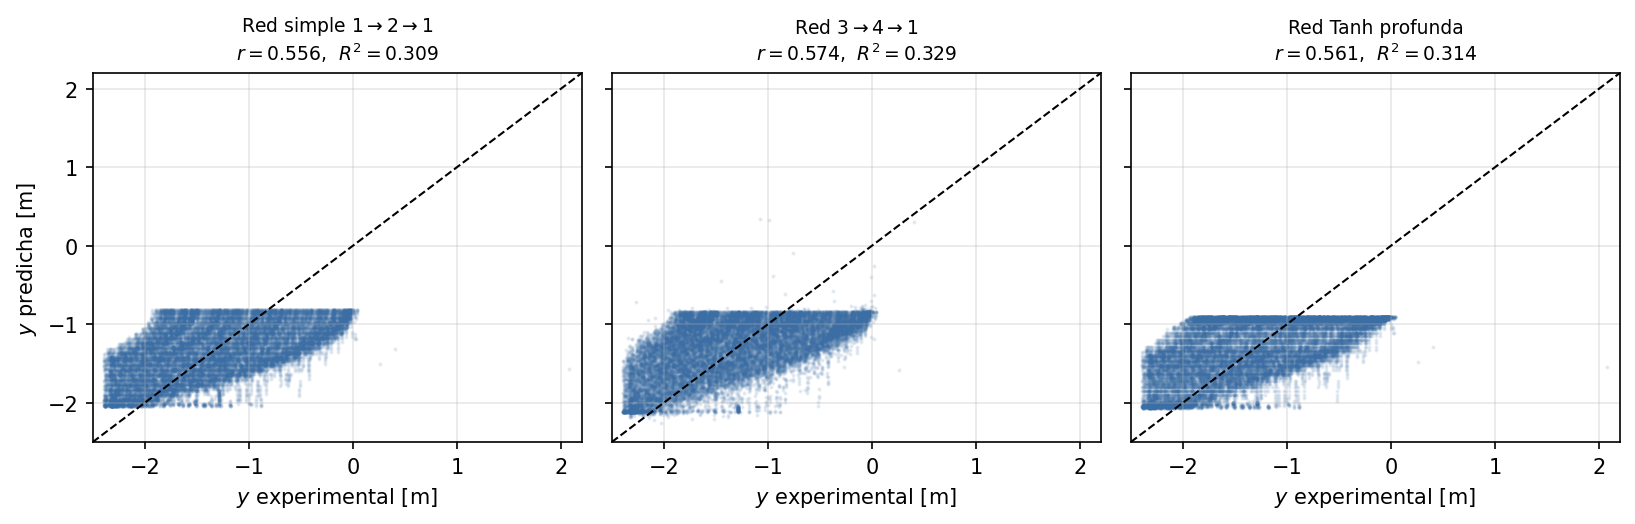
\includegraphics[width=\linewidth]{imgs/pred_vs_real.png}
  \caption{Posición predicha frente a posición experimental para las tres
    redes. La línea discontinua es la identidad. El estrechamiento vertical de
    la nube respecto de su extensión horizontal indica que las redes comprimen
    la variabilidad de los datos hacia un valor medio.}
  \label{fig:predvsreal}
\end{figure}

\subsection{Recuperación de $g$: el ajuste agregado no es una prueba válida}
\label{subsec:agregado}

Aplicando el ajuste cuadrático sobre el conjunto agregado, tal como se hizo en
la primera versión del análisis, se obtienen los valores de la
tabla~\ref{tab:agregado}.

\begin{table}[H]
  \centering
  \begin{tabular}{lrrr}
    \toprule
    Modelo & $g_{\text{pred}}$ & $g_{\text{ref}}$ & Diferencia \\
    \midrule
    Red $3\to4\to1$        & $-0.3564$ & $-0.3500$ & $-0.0064$ \\
    Red $\tanh$ profunda   & $-0.3570$ & $-0.3500$ & $-0.0070$ \\
    Red simple $1\to2\to1$ & $-0.3438$ & $-0.3500$ & $+0.0062$ \\
    \bottomrule
  \end{tabular}
  \caption{Estimación de $g$ (en \meter\per\second\squared) mediante un único
    ajuste cuadrático sobre los \num{20\,210} puntos agregados. Las diferencias
    con el valor de referencia son inferiores al \SI{2}{\percent}, pero
    \emph{ese valor de referencia no es la aceleración de la gravedad}.}
  \label{tab:agregado}
\end{table}

Leída sin más contexto, esta tabla sugiere un acuerdo excelente: las tres redes
reproducen el coeficiente de referencia con menos del \SI{2}{\percent} de
discrepancia. La conclusión es, sin embargo, incorrecta, y la razón está a la
vista en el propio valor de referencia:
$g_{\text{ref}}=\num{-0.35}~\meter\per\second\squared$ difiere del valor
esperado $\num{-9.81}~\meter\per\second\squared$ en un factor de 28.

El origen del problema se ilustra en la figura~\ref{fig:agregado}. Cada clip
tiene su propio origen temporal, heredado del video del que se extrajo, de modo
que los \num{20\,210} puntos se reparten sobre un intervalo de
$0$ a \unit{10.4}{\second} aunque cada trayectoria individual dure apenas
\unit{0.54}{\second} en promedio. Además, cada clip parte de una altura
inicial distinta. La parábola que mejor ajusta esa nube heterogénea es una
curva que no pasa cerca de ningún dato real --- alcanza su vértice en
$t\approx\unit{5.2}{\second}$, donde no hay observaciones --- y su coeficiente
$c_2$ no tiene nada que ver con la gravedad. Es, simplemente, el número que
minimiza el error sobre una mezcla de trayectorias incompatibles entre sí.

\begin{figure}[H]
  \centering
  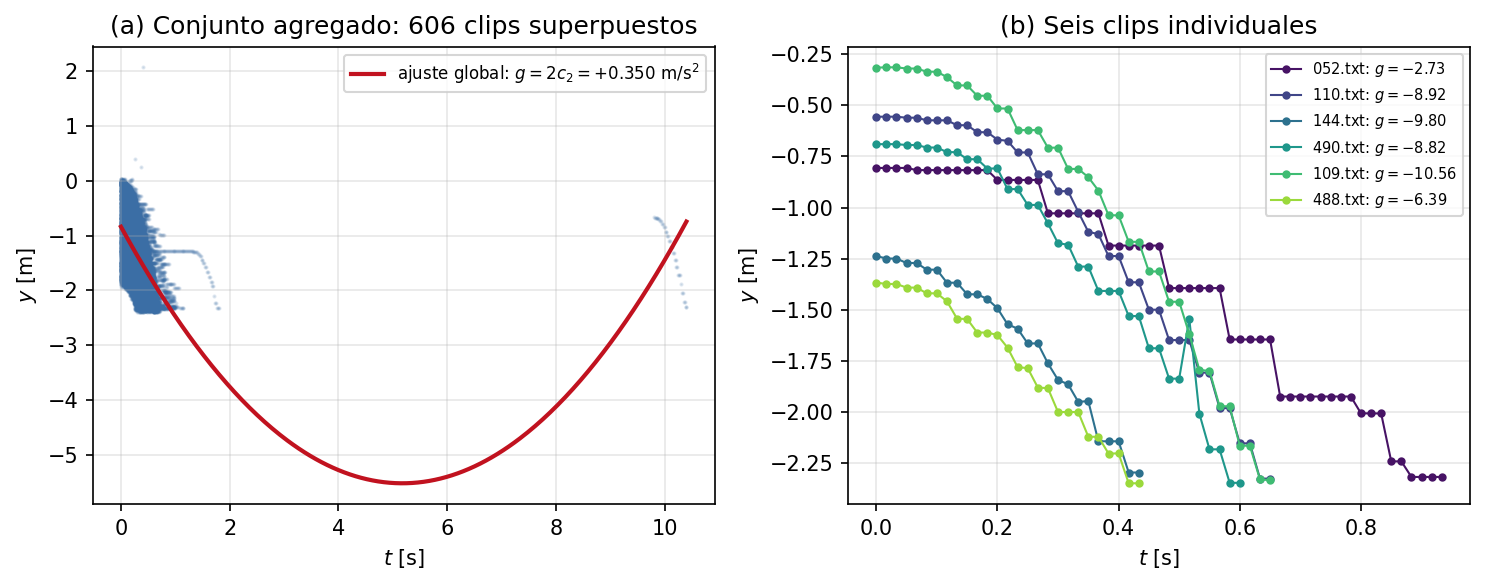
\includegraphics[width=\linewidth]{imgs/agregado_vs_clip.png}
  \caption{(a) Los \num{20\,210} puntos experimentales superpuestos y la parábola
    ajustada al conjunto agregado. La curva ajustada se aleja de los datos, que
    se concentran en $t<\unit{1}{\second}$, y su coeficiente cuadrático
    corresponde a $g=+\num{0.350}~\meter\per\second\squared$, sin significado
    físico. (b) Seis clips individuales; cada uno tiene su propia altura
    inicial y un ajuste parabólico propio con $g$ del orden de
    $\num{-9}~\meter\per\second\squared$.}
  \label{fig:agregado}
\end{figure}

En consecuencia, el acuerdo de la tabla~\ref{tab:agregado} no mide comprensión
física. Mide que las redes y el ajuste agregado están cometiendo el mismo error
sobre los mismos datos mal combinados, lo cual era de esperar y no aporta
información. El criterio de validación debe aplicarse clip por clip.

\subsection{Recuperación de $g$ clip por clip}
\label{subsec:porclip}

Al ajustar una parábola independiente a cada uno de los 606 clips el panorama
cambia por completo. La tabla~\ref{tab:porclip} recoge la estadística de esas
606 estimaciones para los datos experimentales y para las predicciones de cada
red.

\begin{table}[H]
  \centering
  \begin{tabular}{lrrr}
    \toprule
    Fuente & Media & Mediana & Desv.\ est. \\
    \midrule
    \textbf{Datos experimentales}   & $\mathbf{-9.00}$ & $\mathbf{-9.38}$ & $2.36$ \\
    \midrule
    Red $3\to4\to1$        & $-3.25$ & $-2.99$ & $2.41$ \\
    Red $\tanh$ profunda   & $-3.60$ & $-2.89$ & $2.80$ \\
    Red simple $1\to2\to1$ & $+0.17$ & $-0.00$ & $0.59$ \\
    \bottomrule
  \end{tabular}
  \caption{Estadística de las 606 estimaciones de $g$
    (\meter\per\second\squared) obtenidas ajustando una parábola por clip. El
    valor de referencia físico es
    $\num{-9.81}~\meter\per\second\squared$.}
  \label{tab:porclip}
\end{table}

Los datos experimentales superan la prueba: la mediana de
$\num{-9.38}~\meter\per\second\squared$ está a un \SI{4}{\percent} del valor
esperado, lo que confirma que el montaje experimental y la digitalización con
\emph{Tracker} son adecuados y que la información física \emph{está presente en
los datos}. La dispersión de $\num{2.36}~\meter\per\second\squared$ es
apreciable y se atribuye a la corta duración de cada clip --- media
\unit{0.54}{\second}, unos 33 puntos --- combinada con la resolución espacial
del seguimiento; en la figura~\ref{fig:agregado}(b) se aprecia el escalonado
característico de la cuantización a nivel de píxel, que afecta más al
coeficiente cuadrático que a los de orden inferior.

Las redes, en cambio, no la superan. Las dos mejores recuperan alrededor de un
tercio del valor correcto, y la red simple $1\to2\to1$ devuelve
esencialmente cero: sus predicciones dentro de cada clip son casi una recta, de
modo que el coeficiente cuadrático se anula. La
figura~\ref{fig:histg} muestra las distribuciones completas y hace evidente que
no se trata de un sesgo pequeño sino de dos poblaciones separadas.

\begin{figure}[H]
  \centering
  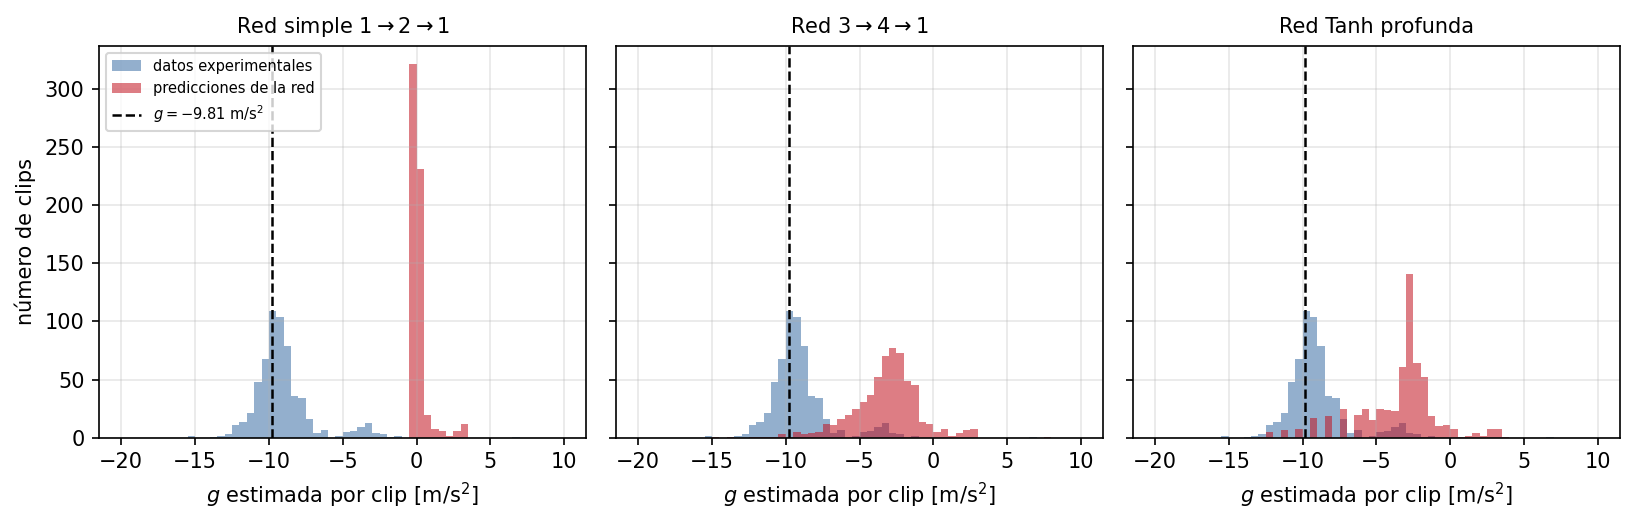
\includegraphics[width=\linewidth]{imgs/hist_g_por_clip.png}
  \caption{Distribución de las 606 estimaciones de $g$ por clip. En azul, las
    obtenidas de los datos experimentales, centradas cerca del valor esperado
    (línea discontinua). En rojo, las obtenidas de las predicciones de cada
    red. La red simple concentra toda su masa en $g\approx0$; las otras dos
    alcanzan aproximadamente un tercio del valor correcto.}
  \label{fig:histg}
\end{figure}

Corresponde por tanto corregir la conclusión que se había extraído del ajuste
agregado: \textbf{ninguna de las tres redes infiere el modelo físico de la
caída libre}. El acuerdo aparente de la tabla~\ref{tab:agregado} era un
artefacto del protocolo de evaluación.

\subsection{Diagnóstico: el problema no es identificable tal como se planteó}
\label{subsec:identificabilidad}

La causa del fracaso no está en las arquitecturas ni en el entrenamiento, sino
en la formulación del problema de aprendizaje, y se sigue de la tercera
observación de la sección~\ref{subsec:mru}.

Al concatenar los 606 clips y pedir a la red que aprenda un mapeo $y=f(t)$, se
está exigiendo que un único valor de entrada produzca un único valor de salida.
Pero en el conjunto de entrenamiento hay, para cada instante $t$ del rango
útil, decenas de puntos procedentes de clips distintos con alturas iniciales
distintas: el mismo $t$ aparece asociado a valores de $y$ que difieren en más
de un metro. Ninguna función puede satisfacer simultáneamente todas esas
restricciones. El problema es no identificable en el sentido de la
sección~\ref{subsubsec:identificabilidad-teoria}.

Lo que sigue es entonces predecible. Al minimizar el error cuadrático, la
solución óptima es la media condicional
$f^\star(t)=\mathbb{E}[y\mid t]$ de la
ecuación~\eqref{eq:mediacondicional}: para cada instante, el promedio de las
posiciones de todos los clips en ese instante. Como los clips no están
sincronizados ni comparten altura inicial, ese promedio es una curva suave y
casi lineal que no corresponde a ninguna trayectoria real y cuyo coeficiente
cuadrático es próximo a cero. Es exactamente lo que devuelven las redes.

La figura~\ref{fig:trayectorias} confirma el diagnóstico de la manera más
directa. En los cuatro clips mostrados, las tres redes producen prácticamente
la \emph{misma} curva, independientemente del clip: no pueden hacer otra cosa,
porque su única entrada es $t$ y todos los clips comienzan en $t=0$. Cuando la
altura inicial del clip coincide aproximadamente con la media del conjunto
(paneles tercero y cuarto) la predicción parece razonable; cuando no coincide
(paneles primero y segundo) el desfase es de casi un metro. Esa es la fuente
del RMSE de \num{0.51}~\meter\ y del $R^2$ de \num{0.31}.

\begin{figure}[H]
  \centering
  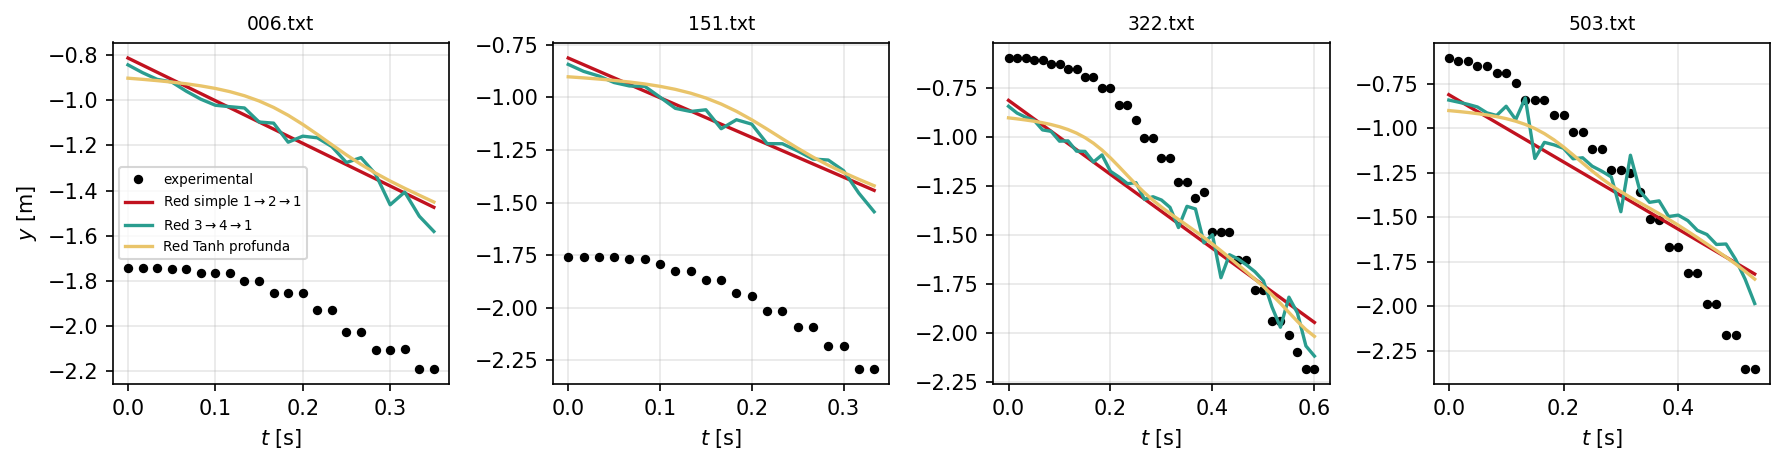
\includegraphics[width=\linewidth]{imgs/trayectorias_ejemplo.png}
  \caption{Cuatro clips experimentales (puntos negros) con las predicciones de
    las tres redes superpuestas. Las predicciones son casi idénticas entre
    clips, porque la entrada $t$ no distingue un clip de otro. El desajuste
    vertical en los dos primeros paneles corresponde a clips cuya altura
    inicial se aparta de la media del conjunto.}
  \label{fig:trayectorias}
\end{figure}

Esto explica también por qué la red $3\to4\to1$ es la única que se acerca algo
al valor correcto. Sus entradas $v_y$ y $a_y$ sí distinguen un clip de otro:
codifican el estado dinámico instantáneo y, en principio, permiten reconstruir
la trayectoria. La red aprovecha esa información y pasa de $g\approx0$ a
$g\approx\num{-3}~\meter\per\second\squared$. No llega más lejos por dos
motivos: $v_y$ y $a_y$ son derivadas numéricas obtenidas por diferencias
finitas y por tanto mucho más ruidosas que las posiciones --- particularmente
$a_y$, que es una segunda derivada ---, y una capa oculta de cuatro unidades
ReLU no tiene capacidad para representar los productos y composiciones que
exigiría la reconstrucción exacta. La mejora observada es, en cualquier caso,
consistente con el diagnóstico: suministrar información que identifique el clip
es lo que hace avanzar el resultado.

Por el mismo argumento se entiende que la red $\tanh$ profunda, con
\num{1153} parámetros frente a los 7 de la red simple, no supere de forma clara
a la red $3\to4\to1$, que tiene 21. Cuando el límite es de identificabilidad y
no de capacidad, añadir parámetros no ayuda: la red $\tanh$ simplemente aprende
la media condicional con mayor fidelidad, lo que la acerca a un $R^2$ ligeramente
distinto pero no le permite recuperar $g$.

\subsection{Efecto del número de épocas}
\label{subsec:epocas}

La tabla~\ref{tab:epochs} recoge el estudio del número de épocas y la
figura~\ref{fig:epochs_comparison} lo resume gráficamente.

\begin{table}[H]
  \centering
  \begin{tabular}{lrrrr}
    \toprule
    Modelo & Épocas & Tiempo [\second] & RMSE [\meter] & MAE [\meter] \\
    \midrule
    \multirow{7}{*}{Red simple $1\to2\to1$} & 10 & 3.15 & 0.6749 & 0.5760 \\
    & 20 & 2.60 & 0.6061 & 0.5114 \\
    & 50 & 8.64 & 0.5236 & 0.4479 \\
    & 100 & 14.81 & 0.6186 & 0.5223 \\
    & 200 & 29.12 & 0.6029 & 0.5060 \\
    & 400 & 59.14 & 0.5126 & 0.4332 \\
    & 700 & 101.86 & 0.6029 & 0.5061 \\
    \midrule
    \multirow{7}{*}{Red $3\to4\to1$} & 10 & 1.46 & 0.5874 & 0.4932 \\
    & 20 & 2.90 & 0.5571 & 0.4724 \\
    & 50 & 7.50 & 0.5117 & 0.4319 \\
    & 100 & 14.57 & 0.5096 & 0.4304 \\
    & 200 & 32.08 & 0.5073 & 0.4268 \\
    & 400 & 59.87 & 0.5106 & 0.4307 \\
    & 700 & 100.69 & 0.5064 & 0.4265 \\
    \midrule
    \multirow{7}{*}{Red $\tanh$ profunda} & 10 & 1.76 & 0.5164 & 0.4360 \\
    & 20 & 3.13 & 0.5134 & 0.4347 \\
    & 50 & 8.37 & 0.5130 & 0.4336 \\
    & 100 & 16.44 & 0.5129 & 0.4336 \\
    & 200 & 32.63 & 0.5129 & 0.4340 \\
    & 400 & 67.43 & 0.5122 & 0.4324 \\
    & 700 & 109.56 & 0.5121 & 0.4322 \\
    \bottomrule
  \end{tabular}
  \caption{Impacto del número de épocas en RMSE, MAE y tiempo de entrenamiento.
    Cada fila es un entrenamiento independiente con inicialización aleatoria
    propia.}
  \label{tab:epochs}
\end{table}

\begin{figure}[H]
  \centering
  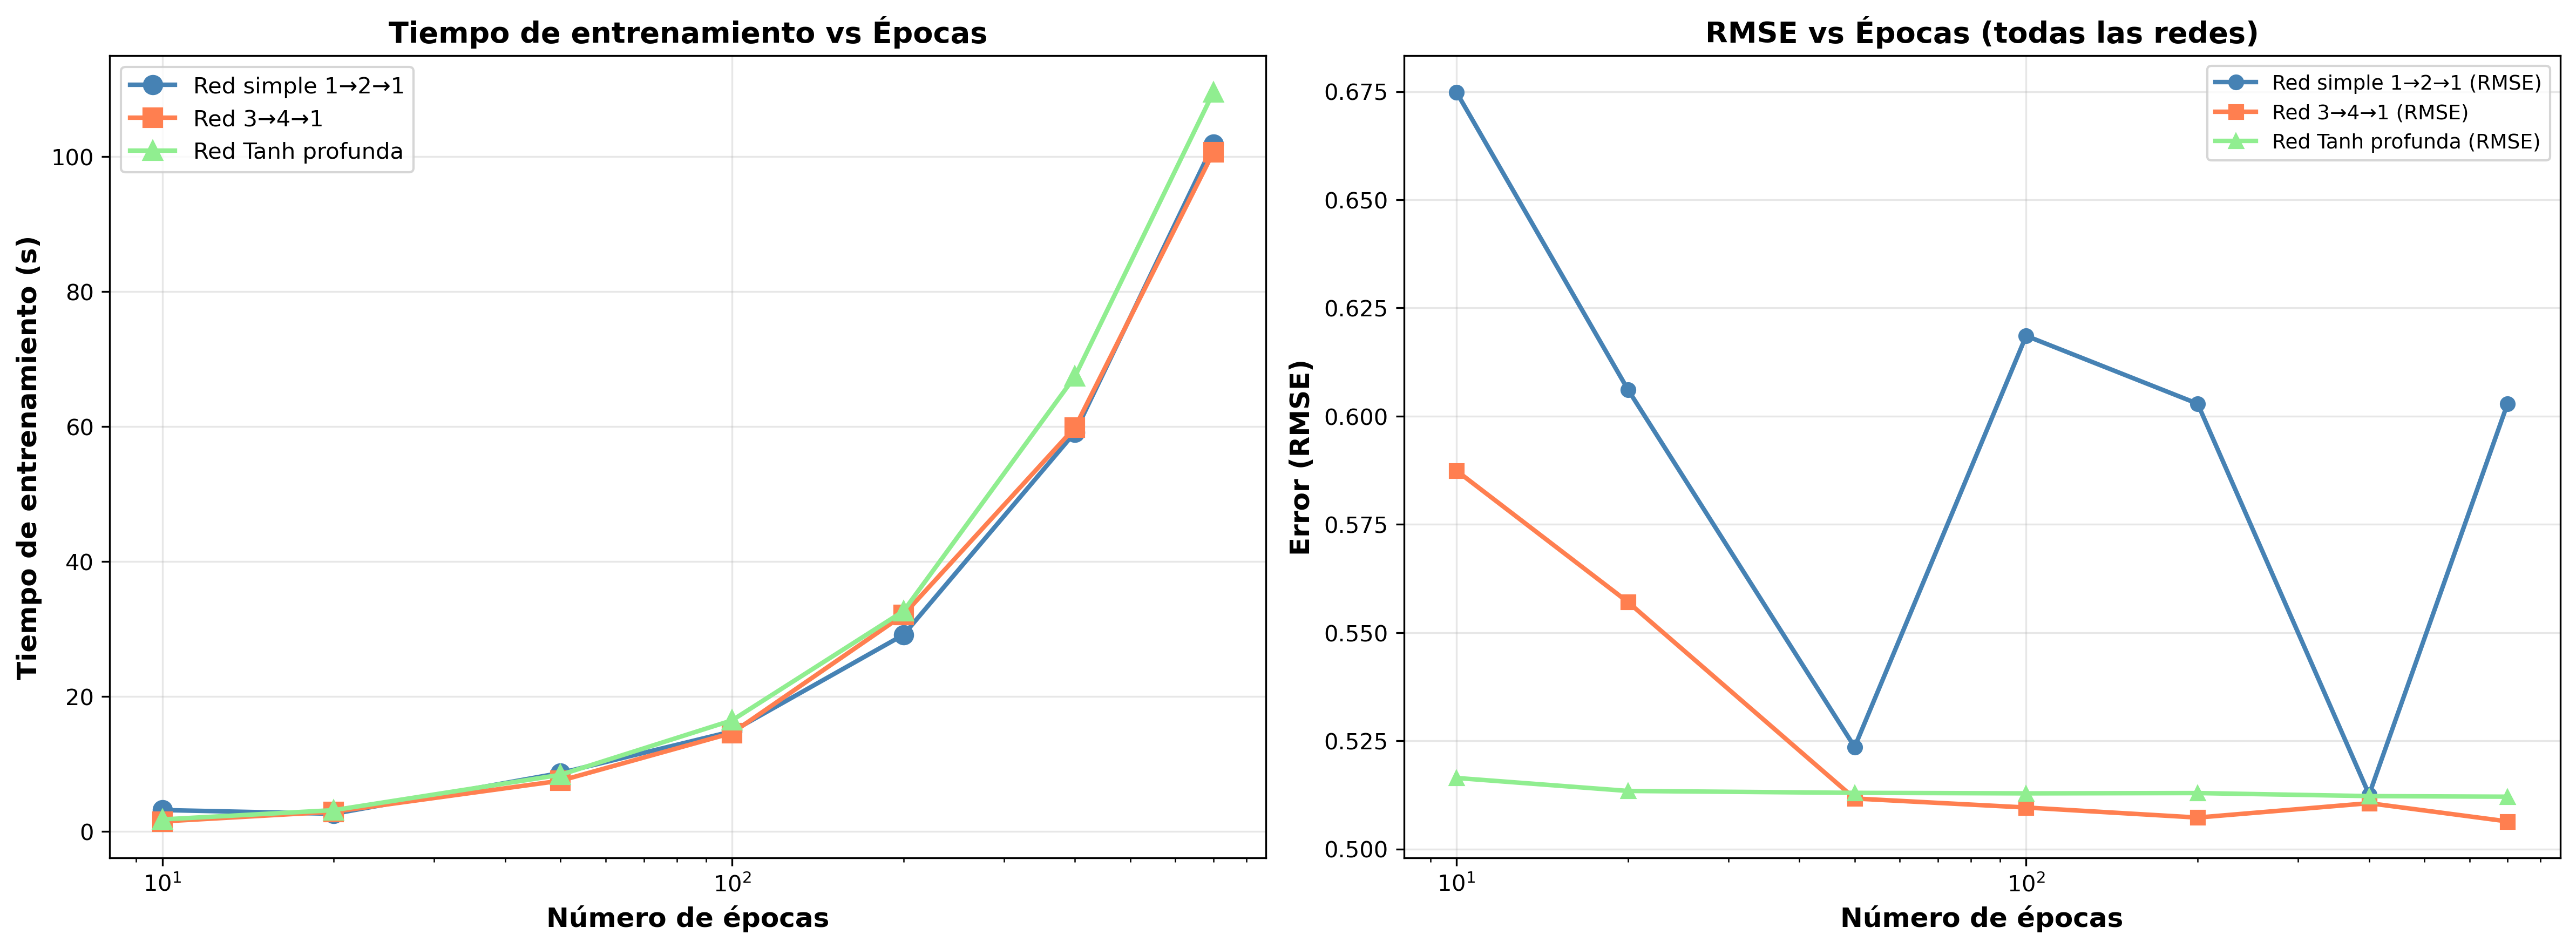
\includegraphics[width=\linewidth]{imgs/epochs_analysis_all_models.png}
  \caption{Tiempo de entrenamiento frente a épocas (izquierda) y RMSE frente a
    épocas (derecha) para las tres redes evaluadas.}
  \label{fig:epochs_comparison}
\end{figure}

\begin{figure}[H]
  \centering
  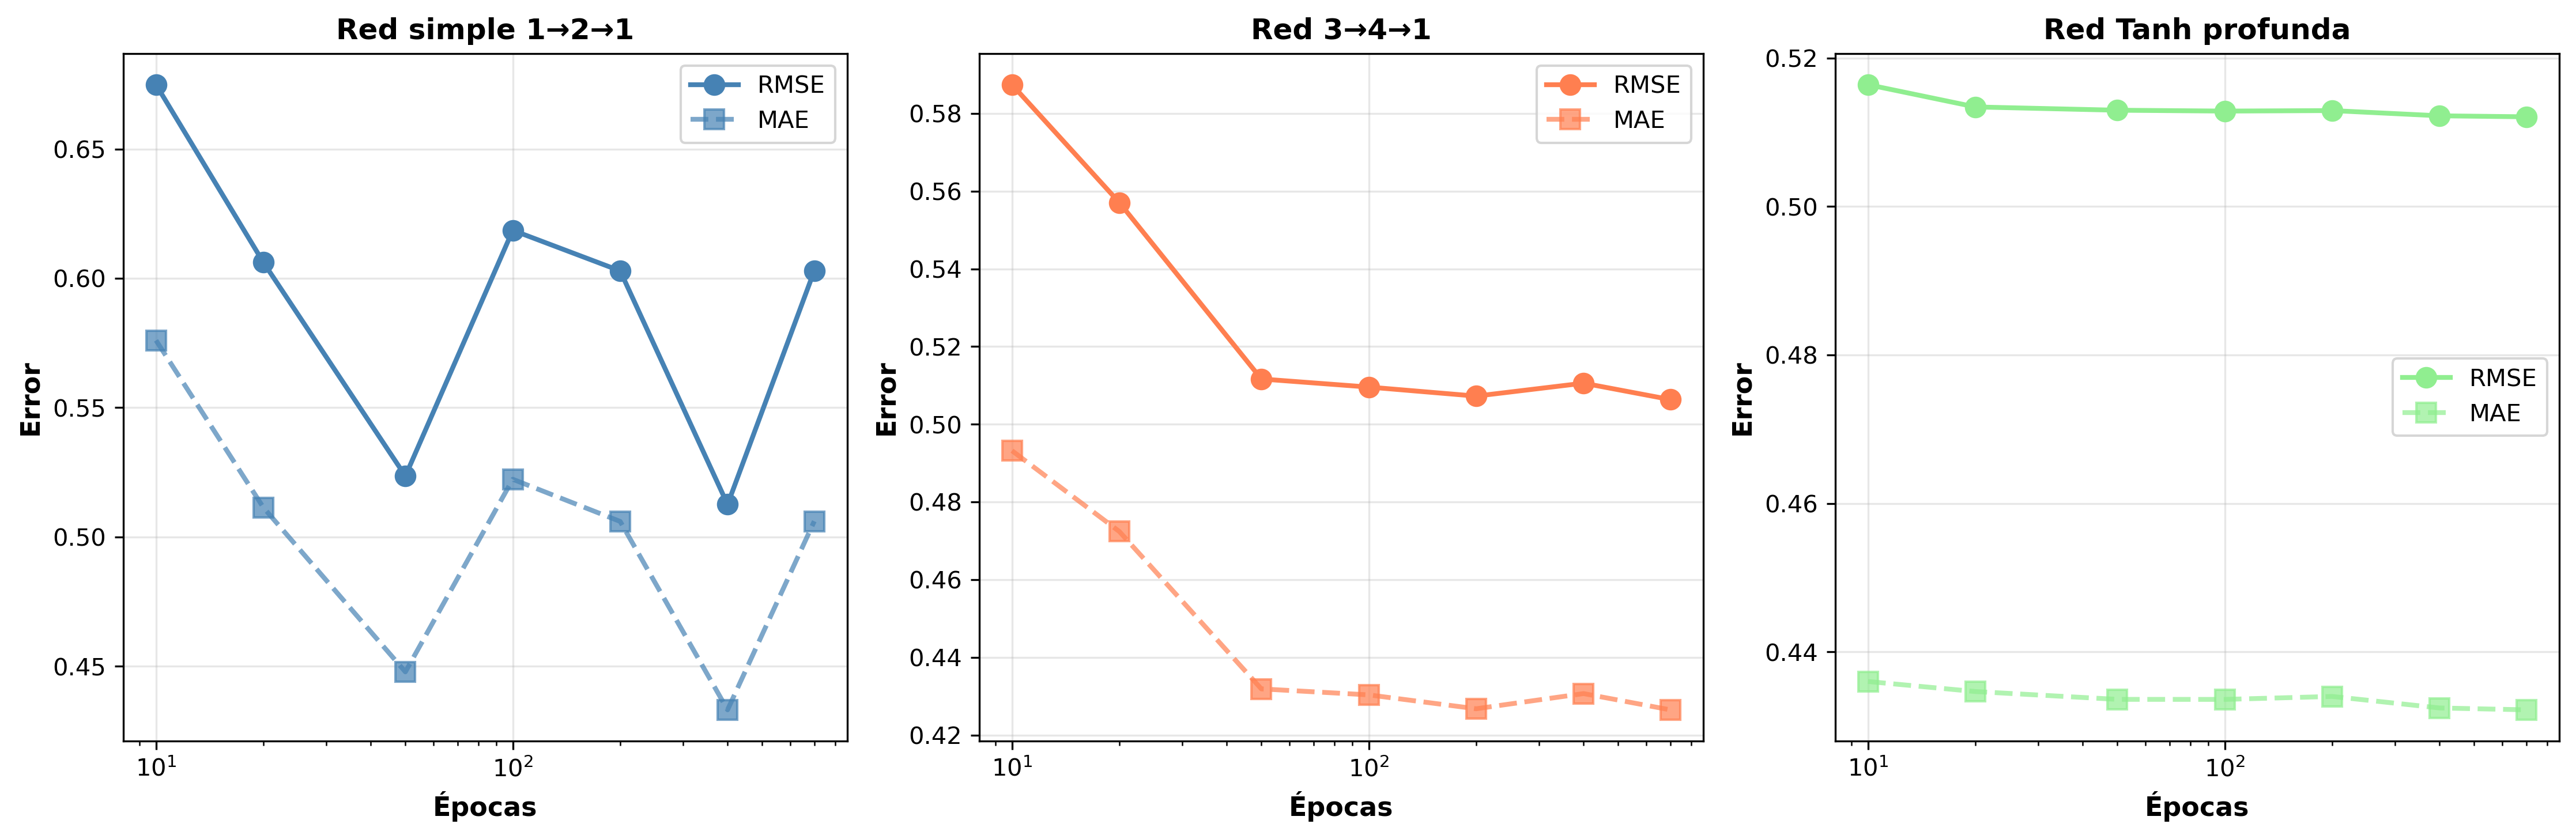
\includegraphics[width=\linewidth]{imgs/epochs_analysis_individual.png}
  \caption{Gráficos individuales de RMSE y MAE frente al número de épocas para
    cada red. Se observa la oscilación de la red simple (izquierda), la
    convergencia progresiva de la red $3\to4\to1$ (centro) y la convergencia
    temprana de la red $\tanh$ (derecha).}
  \label{fig:epochs_individual}
\end{figure}

Tres observaciones.

\paragraph{La red $\tanh$ converge de inmediato.} A partir de 50 épocas su RMSE
es prácticamente invariante (\num{0.5130} frente a \num{0.5121} en 700 épocas,
una diferencia del \SI{0.2}{\percent} a costa de trece veces más cómputo). Esto
es coherente con la interpretación de la
sección~\ref{subsec:identificabilidad}: la media condicional es una función
suave y fácil de aproximar, y una vez alcanzada no hay nada más que aprender.
El estancamiento no es un límite de la red, es el suelo de error impuesto por
la varianza condicional de los datos.

\paragraph{La red $3\to4\to1$ mejora de forma gradual y modesta.} Baja de
\num{0.5874} a \num{0.5064} entre 10 y 700 épocas. Su información adicional le
permite reducir algo el error, pero la curva se aplana rápidamente y la mejora
entre 200 y 700 épocas es inferior al \SI{0.2}{\percent}.

\paragraph{La red simple oscila.} Su RMSE alterna entre \num{0.51} y
\num{0.67} sin tendencia monótona: mejora hasta 50 épocas, empeora a 100,
mejora a 400 y vuelve a empeorar a 700. En la primera versión del análisis esta
oscilación se interpretó como sobreajuste posterior al \enquote{descubrimiento}
de la física. Esa lectura no se sostiene, por dos razones. La primera es que el
sobreajuste produce un patrón distinto --- error de entrenamiento que sigue
bajando mientras el de validación sube de forma sostenida --- y no una
alternancia no monótona. La segunda es que con siete parámetros y \num{20\,210}
muestras el sobreajuste es prácticamente imposible.

La explicación es más simple. Cada fila de la tabla es un entrenamiento
independiente con su propia inicialización aleatoria, y con solo dos neuronas
ocultas ReLU el resultado depende críticamente de esa inicialización: basta con
que una de las dos unidades quede en la región de gradiente nulo --- el
fenómeno de ReLU muerta descrito en la
sección~\ref{subsec:redneuronal} --- para que la red se reduzca de hecho a una
sola neurona. Los valores de RMSE~$\approx\num{0.60}$ y
RMSE~$\approx\num{0.51}$ corresponden verosímilmente a esos dos regímenes. La
oscilación es, por tanto, dispersión entre semillas y no una dinámica de
aprendizaje; comprobarlo requeriría repetir cada configuración con varias
semillas, lo que se recomienda en la sección~\ref{sec:trabajofuturo}.

\subsection{Síntesis de la discusión}

Reuniendo los tres niveles de evidencia:

\begin{itemize}
\item Las tres redes alcanzan un RMSE que mejora solo un \SI{18}{\percent} al
  del predictor constante, con $R^2\approx\num{0.31}$
  (tabla~\ref{tab:metricas}).
\item Los datos experimentales contienen la física buscada: ajustados clip por
  clip dan $g$ con mediana $\num{-9.38}~\meter\per\second\squared$
  (tabla~\ref{tab:porclip}).
\item Las predicciones de las redes, sometidas al mismo ajuste, dan entre
  $\num{0}$ y $\num{-3.6}~\meter\per\second\squared$
  (tabla~\ref{tab:porclip}, figura~\ref{fig:histg}).
\item Las predicciones son casi idénticas para clips distintos
  (figura~\ref{fig:trayectorias}), como corresponde a un modelo que aproxima la
  media condicional.
\end{itemize}

Todo apunta en la misma dirección: las redes aprendieron el promedio de un
conjunto de trayectorias incompatibles entre sí, no la ley que las genera. El
fallo es de planteamiento, no de capacidad, y esa distinción es precisamente
lo que hace que el resultado sea utilizable: indica qué hay que cambiar.

La sección siguiente aplica ese cambio y comprueba si basta.


% % % % % % % % % % % % % % % % % % % % % % % % % % % % % % % % % % %
\section{Verificación del supuesto: reformulación del problema}
\label{sec:v2}

El diagnóstico de la sección~\ref{subsec:identificabilidad} tiene una
consecuencia práctica inmediata: si el fallo es de planteamiento y no de las
redes, entonces corregir el planteamiento debería bastar para que el supuesto
del anteproyecto pueda verificarse. Esta sección lo pone a prueba. Todo el
código correspondiente está en la carpeta \texttt{Proyectov2/} del repositorio
del proyecto.

\subsection{Rediseño del experimento}
\label{subsec:rediseno}

La corrección central es referir cada clip a su propio origen. Con
$\tau = t-t_0$ y $\Delta y = y-y_0$ medidos \emph{dentro} de cada clip, la
ecuación~\eqref{eq:mruv} se convierte en
\begin{equation}
  \Delta y = v_0\,\tau + \frac{1}{2}g\,\tau^2,
  \label{eq:mruv_ref}
\end{equation}
donde $y_0$ ha desaparecido y $g$ es el único parámetro compartido por todas
las trayectorias. La altura inicial, que era la causa de la ambigüedad, deja de
intervenir.

Queda $v_0$. La velocidad inicial no es la misma en todos los clips ---media
$\num{-0.21}~\meter\per\second$, desviación estándar
$\num{0.25}~\meter\per\second$--- porque no todos empiezan en el instante exacto
de la soltada. Sin $v_0$ el problema sigue siendo parcialmente ambiguo, así que
se incluye como segunda entrada. Se estima con un ajuste lineal a los
\emph{tres primeros puntos} de cada clip: \emph{Tracker} no proporciona
velocidad en el primer fotograma, y usar solo el arranque evita que la
estimación absorba la curvatura, que es justamente lo que se quiere medir
después.

Para no dar por supuesto el efecto de cada cambio, se evalúan tres
formulaciones:

\begin{description}
\item[\texttt{v1}:] $t\to y$, clips concatenados. Reproduce el planteamiento
  original y sirve de control.
\item[\texttt{tau}:] $\tau\to\Delta y$. Solo el cambio de origen.
\item[\texttt{tau\_v0}:] $(\tau,v_0)\to\Delta y$. Formulación identificable
  completa.
\end{description}

El resto del protocolo se corrigió según las limitaciones detectadas en la
sección~\ref{sec:limitaciones}. La tabla~\ref{tab:v1v2} resume las diferencias.

\begin{table}[H]
  \centering
  \begin{tabular}{lll}
    \toprule
    & Versión inicial & Versión corregida \\
    \midrule
    Formulación   & $t\to y$, clips concatenados & $(\tau,v_0)\to\Delta y$ \\
    Partición     & \SI{80}{\percent}/\SI{20}{\percent} por \emph{punto}
                  & por \emph{clip} completo, 70/15/15 \\
    Normalización & sobre todo el conjunto & solo con clips de entrenamiento \\
    Semillas      & 1 & 5, con media y desviación \\
    Parada        & número fijo de épocas & temprana, sobre clips no vistos \\
    Líneas base   & ninguna & tres (véase sección~\ref{subsec:v2_error}) \\
    Estimación de $g$ & un ajuste sobre el agregado & un ajuste \emph{por clip} \\
    Calidad de datos & sin filtro & descarta residuo $>\unit{8}{\centi\meter}$ \\
    \bottomrule
  \end{tabular}
  \caption{Diferencias de protocolo entre la formulación inicial y la
    corregida. Las arquitecturas de red son deliberadamente las mismas, de modo
    que cualquier cambio en el resultado provenga del planteamiento del
    problema y no de haber usado redes distintas.}
  \label{tab:v1v2}
\end{table}

El filtro de calidad descarta los clips cuyo ajuste parabólico deja un residuo
superior a \unit{8}{\centi\meter}, que corresponden a fallos de seguimiento de
\emph{Tracker} y no a trayectorias físicamente distintas. Elimina 25 de los 606
clips (\SI{4}{\percent}) y deja \num{581} clips con \num{18\,992} muestras. Sobre
ese conjunto la referencia experimental es
\begin{equation}
  g_{\text{exp}} = \num{-9.43}~\meter\per\second\squared \quad
  \text{(mediana del ajuste por clip)},
\end{equation}
a un \SI{3.9}{\percent} del valor físico $\num{-9.81}~\meter\per\second\squared$.
Esa diferencia es un sesgo del montaje experimental, y conviene tenerla presente:
\textbf{una red no puede recuperar más física de la que los datos contienen}, de
modo que el criterio de éxito es acercarse a $g_{\text{exp}}$, no a
$\num{-9.81}$.

Se entrenaron las tres formulaciones con las tres arquitecturas de la
sección~\ref{subsec:arquitecturas} y cinco semillas distintas, en total 45
entrenamientos, con optimizador Adam, $\eta=10^{-2}$, hasta 800 épocas y parada
temprana sobre clips de validación completos.

\subsection{Recuperación del parámetro físico}
\label{subsec:v2_g}

La tabla~\ref{tab:v2g} recoge el resultado principal.

\begin{table}[H]
  \centering
  \begin{tabular}{llrrr}
    \toprule
    Formulación & Arquitectura & Parámetros & $g$ recuperada & Error vs.\ $-9.81$ \\
    \midrule
    \multirow{3}{*}{\texttt{v1}}
      & simple $(2)$    & 7    & $+0.00 \pm 0.00$ & \SI{100.0}{\percent} \\
      & media $(4)$     & 13   & $-1.21 \pm 1.67$ & \SI{87.6}{\percent} \\
      & tanh $32\times32$ & 1153 & $-2.77 \pm 0.56$ & \SI{71.8}{\percent} \\
    \midrule
    \multirow{3}{*}{\texttt{tau}}
      & simple $(2)$    & 7    & $-3.02 \pm 4.14$ & \SI{69.2}{\percent} \\
      & media $(4)$     & 13   & $-7.61 \pm 0.39$ & \SI{22.5}{\percent} \\
      & tanh $32\times32$ & 1153 & $-9.07 \pm 0.28$ & \SI{7.6}{\percent} \\
    \midrule
    \multirow{3}{*}{\texttt{tau\_v0}}
      & simple $(2)$    & 9    & $-4.68 \pm 4.30$ & \SI{52.3}{\percent} \\
      & media $(4)$     & 17   & $-7.53 \pm 0.57$ & \SI{23.3}{\percent} \\
      & \textbf{tanh $32\times32$} & 1185 & $\mathbf{-9.46 \pm 0.33}$
        & \textbf{\SI{3.8}{\percent}} \\
    \midrule
    \multicolumn{3}{l}{\emph{Referencia experimental} (ajuste por clip)}
      & $-9.48 \pm 0.11$ & \SI{3.4}{\percent} \\
    \bottomrule
  \end{tabular}
  \caption{Mediana de la $g$ recuperada ajustando una parábola a las
    predicciones de cada clip de prueba, en \meter\per\second\squared. Media y
    desviación estándar sobre cinco semillas, evaluadas siempre sobre clips que
    la red no vio durante el entrenamiento.}
  \label{tab:v2g}
\end{table}

El resultado es inequívoco. Con la formulación original, la mejor de las tres
redes se queda en $\num{-2.77}~\meter\per\second\squared$, un
\SI{72}{\percent} de error. Con la formulación corregida, la misma red alcanza
$\num{-9.46}\pm\num{0.33}~\meter\per\second\squared$.

La comparación pertinente no es contra $\num{-9.81}$ sino contra la referencia
experimental $g_{\text{exp}}=\num{-9.48}$, que es lo que el método clásico
extrae de estos mismos datos: la discrepancia es entonces de
\textbf{\SI{0.2}{\percent}}. La red reproduce la gravedad contenida en el
conjunto de datos prácticamente sin sesgo; el \SI{3.4}{\percent} restante
frente al valor verdadero es una limitación del experimento, común a la red y
al método clásico.

La figura~\ref{fig:v2_form} presenta el mismo resultado gráficamente y la
figura~\ref{fig:v2_hist} muestra las distribuciones completas: bajo
\texttt{v1} las dos poblaciones están separadas, bajo \texttt{tau\_v0} se
superponen.

\begin{figure}[H]
  \centering
  
\includegraphics[width=\linewidth]{imgs/v2/01_formulaciones.png}
  \caption{(a) Gravedad recuperada por formulación y arquitectura; la línea
    discontinua es el valor físico. (b) RMSE sobre clips no vistos, con las
    tres líneas base como referencia. Barras de error: desviación estándar
    sobre cinco semillas.}
  \label{fig:v2_form}
\end{figure}

\begin{figure}[H]
  \centering
  
\includegraphics[width=\linewidth]{imgs/v2/02_g_por_clip.png}
  \caption{Distribución de la $g$ estimada clip por clip para la red
    $\tanh$ $32\times32$, en azul la de los datos experimentales y en color la
    de las predicciones. Al pasar de \texttt{v1} a \texttt{tau\_v0} las dos
    distribuciones dejan de estar separadas y se superponen.}
  \label{fig:v2_hist}
\end{figure}

La figura~\ref{fig:v2_tray} es quizá la más clara de todo el informe. En la
fila superior, la red bajo la formulación original produce la misma curva para
los cuatro clips, con desajustes de hasta un metro. En la inferior, la misma
arquitectura bajo la formulación corregida sigue la parábola de cada clip.

\begin{figure}[H]
  \centering
  
\includegraphics[width=\linewidth]{imgs/v2/03_trayectorias.png}
  \caption{Cuatro clips de prueba con las predicciones de la red
    $\tanh$ $32\times32$. Arriba, formulación \texttt{v1}: la red no puede
    distinguir un clip de otro y predice esencialmente la misma curva para
    todos. Abajo, formulación \texttt{tau\_v0}: la red reproduce la trayectoria
    de cada clip.}
  \label{fig:v2_tray}
\end{figure}

\subsection{Error de predicción y líneas base}
\label{subsec:v2_error}

Para que el RMSE signifique algo se comparó contra tres referencias, de la más
débil a la más fuerte: el predictor constante que devuelve siempre la media; el
modelo físico $\Delta y = v_0\tau + \tfrac{1}{2}g\tau^2$ con una única $g$
ajustada sobre los clips de entrenamiento, es decir, la ecuación de MRUV con un
solo parámetro libre; y el ajuste parabólico independiente por clip, que usa el
propio clip que evalúa y por tanto no es un predictor honesto, pero marca el
suelo de error alcanzable.

\begin{table}[H]
  \centering
  \begin{tabular}{lrrr}
    \toprule
    Modelo & RMSE [\meter] & MAE [\meter] & $R^2$ \\
    \midrule
    Predictor constante $\bar y$          & 0.5534 & --- & 0.000 \\
    Red \texttt{v1}, $\tanh$ $32\times32$ & 0.4970 & 0.4170 & 0.329 \\
    \midrule
    MRUV con $g$ global (1 parámetro)     & 0.2020 & 0.0841 & 0.841 \\
    Red \texttt{tau}, $\tanh$ $32\times32$    & 0.1670 & 0.0984 & 0.898 \\
    \textbf{Red \texttt{tau\_v0}, $\tanh$ $32\times32$} & \textbf{0.1420}
      & \textbf{0.0728} & \textbf{0.926} \\
    \midrule
    Ajuste por clip (oráculo, 3 parám./clip) & 0.0401 & 0.0286 & 0.994 \\
    Suelo de ruido (residuo del ajuste)      & 0.0343 & --- & --- \\
    \bottomrule
  \end{tabular}
  \caption{Error de predicción sobre clips no vistos, promediado sobre cinco
    semillas. Todas las cantidades en metros.}
  \label{tab:v2rmse}
\end{table}

Tres observaciones.

\paragraph{El salto es de un factor 3.5.} El RMSE baja de
\num{0.497} a \num{0.142}~\meter\ y el $R^2$ sube de \num{0.33} a \num{0.93}.
Bajo la formulación original las redes explicaban un tercio de la varianza; bajo
la corregida explican el \SI{93}{\percent}.

\paragraph{La red supera al modelo físico analítico.} La ecuación de MRUV con
$g$ global alcanza RMSE~$=\num{0.202}~\meter$; la red llega a
$\num{0.142}~\meter$, un \SI{30}{\percent} mejor con las mismas entradas. La
razón más probable es que $v_0$, estimado a partir de tres puntos ruidosos,
lleva un sesgo sistemático que la red aprende a compensar y que la fórmula
analítica no puede corregir. Este es el primer resultado del proyecto en el que
la red aporta algo que el método clásico no da.

\paragraph{Aún queda margen.} El oráculo por clip alcanza
$\num{0.040}~\meter$, cerca del suelo de ruido de $\num{0.034}~\meter$. La
diferencia con el $\num{0.142}~\meter$ de la red se explica porque el oráculo
ajusta tres parámetros \emph{por clip}, mientras que la red dispone únicamente
de $(\tau,v_0)$ y no puede reproducir las desviaciones individuales de cada
trayectoria.

\subsection{El límite cambia de naturaleza}
\label{subsec:v2_capacidad}

Hay un contraste en las tablas~\ref{tab:v2g} y~\ref{tab:v2rmse} que merece
atención propia, porque constituye la confirmación más fuerte del diagnóstico
de la sección~\ref{subsec:identificabilidad}.

Bajo la formulación \texttt{v1}, pasar de 7 a \num{1153} parámetros
---un factor 165--- apenas mejoraba nada: el RMSE bajaba de \num{0.537} a
\num{0.497}~\meter\ y la $g$ seguía siendo inservible. Bajo \texttt{tau\_v0},
la misma escalada lleva la $g$ recuperada de $\num{-4.68}$ a $\num{-9.46}$ y el
RMSE de \num{0.177} a \num{0.142}~\meter.

Es decir: \textbf{con el problema mal planteado, la capacidad no importaba; con
el problema bien planteado, la capacidad pasa a ser el factor decisivo.} Eso es
exactamente lo que predice el análisis de identificabilidad. Cuando el límite es
de información, ninguna arquitectura puede superarlo, porque la solución óptima
---la media condicional--- ya está al alcance de una red pequeña. Cuando el
límite es de representación, una red mayor sí ayuda.

El fracaso de la red $1\to2\to1$ bajo \texttt{tau\_v0} ($g=\num{-4.68}$, con una
dispersión entre semillas de $\num{4.30}$) tiene ahora una lectura distinta a la
de la sección~\ref{subsec:epocas}: dos unidades ReLU solo pueden formar una
función lineal a trozos con dos quiebres, con la que no se aproxima una
parábola. Es una limitación genuina de capacidad, no un artefacto. La
inestabilidad entre semillas es coherente con el fenómeno de ReLU muerta ya
descrito.

La figura~\ref{fig:v2_scatter} resume las 45 corridas en un solo gráfico.

\begin{figure}[H]
  \centering
  
\includegraphics[width=0.78\linewidth]{imgs/v2/04_rmse_vs_error_g.png}
  \caption{Error relativo en $g$ frente al RMSE para las 45 corridas
    (3 formulaciones $\times$ 3 arquitecturas $\times$ 5 semillas). Las corridas
    con la formulación original se agrupan arriba a la derecha; solo la
    formulación \texttt{tau\_v0} con la red $\tanh$ profunda baja del
    \SI{5}{\percent} de error.}
  \label{fig:v2_scatter}
\end{figure}

\subsection{Síntesis}

El supuesto del anteproyecto \textbf{se verifica}. Una red neuronal entrenada
con datos experimentales de caída libre sí permite recuperar el modelo físico
subyacente, con una discrepancia del \SI{0.2}{\percent} respecto de lo que el
método clásico extrae de los mismos datos.

Lo que hizo falta no fue una red mejor ---son las mismas tres arquitecturas de
la sección~\ref{subsec:arquitecturas}--- ni más datos ---son los mismos 609
clips--- ni más entrenamiento. Hizo falta formular la pregunta de manera que
tuviera respuesta.


% % % % % % % % % % % % % % % % % % % % % % % % % % % % % % % % % % %
\section{Limitaciones del estudio}
\label{sec:limitaciones}

\subsection{Limitaciones de la formulación inicial, ya corregidas}

Las cuatro primeras son defectos de protocolo, y su corrección constituye el
experimento de la sección~\ref{sec:v2}. Se enumeran porque son el objeto de
estudio de la primera mitad del informe, no porque sigan pendientes.

\begin{enumerate}
\item \textbf{No identificabilidad del mapeo $y=f(t)$.} Es la limitación
  principal, discutida en la sección~\ref{subsec:identificabilidad}. Los clips
  se concatenaron sin normalizar el origen temporal ni la altura inicial, de
  modo que la información necesaria para distinguir una trayectoria de otra no
  llegaba a la red. \emph{Corregido} con la formulación $(\tau,v_0)\to\Delta y$
  de la sección~\ref{subsec:rediseno}.

\item \textbf{Partición de validación por punto.} Al repartir los puntos
  individuales al azar, puntos de un mismo clip quedan a ambos lados de la
  partición. El error de validación mide entonces interpolación dentro de clips
  ya vistos y no generalización a un clip nuevo, por lo que sobreestima la
  capacidad del modelo (sección~\ref{subsubsec:sobreajuste}). \emph{Corregido}
  con la partición por clip completo.

\item \textbf{Una sola semilla por configuración.} Sin repeticiones no era
  posible separar las diferencias reales entre arquitecturas de la dispersión
  por inicialización, que en el caso de la red $1\to2\to1$ es del mismo orden
  que las diferencias reportadas (sección~\ref{subsec:epocas}).
  \emph{Corregido} con cinco semillas por configuración.

\item \textbf{Ausencia de una línea base clásica.} No se comparaba contra el
  ajuste cuadrático directo por clip, que es el método convencional para este
  problema. \emph{Corregido} con las tres referencias de la
  sección~\ref{subsec:v2_error}.
\end{enumerate}

\subsection{Limitaciones que permanecen}

Las siguientes son propiedades del conjunto de datos y acotan lo que puede
lograrse con él, con red o sin ella.

\begin{enumerate}
\setcounter{enumi}{4}
\item \textbf{Calidad de la digitalización.} La dispersión de
  $\num{2.36}~\meter\per\second\squared$ en la $g$ experimental por clip y el
  escalonado visible en la figura~\ref{fig:agregado}(b) indican cuantización a
  nivel de píxel. El filtro de calidad de la sección~\ref{subsec:rediseno}
  descarta los peores casos y reduce la dispersión a
  $\num{1.82}~\meter\per\second\squared$, pero no elimina el ruido de fondo.

\item \textbf{Sesgo experimental en $g$.} El método clásico aplicado a estos
  datos da $\num{-9.43}~\meter\per\second\squared$, un \SI{3.9}{\percent} por
  debajo del valor físico. Ese sesgo ---probablemente de calibración de la
  escala espacial o de la velocidad de fotogramas--- afecta por igual a la red
  y al ajuste clásico, y fija el techo de exactitud alcanzable con este
  conjunto.

\item \textbf{Duración de los clips.} Con \unit{0.53}{\second} de media, el
  término cuadrático de la ecuación~\eqref{eq:mruv} contribuye poco frente al
  ruido de medición, lo que hace intrínsecamente difícil estimar $g$ a partir
  de un clip aislado.

\item \textbf{Estimación de $v_0$.} Se obtiene de los tres primeros puntos de
  cada clip y arrastra el ruido de esas mediciones. Que la red supere al modelo
  analítico de MRUV (sección~\ref{subsec:v2_error}) sugiere que compensa un
  sesgo de esa estimación, pero no se comprobó de forma directa.
\end{enumerate}


% % % % % % % % % % % % % % % % % % % % % % % % % % % % % % % % % % %
\section{Conclusiones}
\label{sec:conclusiones}

\begin{enumerate}
\item Se construyó un conjunto de datos experimental propio de caída libre: 609
  clips grabados a \unit{60}{\hertz}, 606 utilizables, \num{20\,210} pares
  $(t,y)$ digitalizados con \emph{Tracker}. El conjunto contiene la física
  buscada, como demuestra el hecho de que un ajuste cuadrático clip por clip
  recupere $g$ con mediana $\num{-9.38}~\meter\per\second\squared$, a un
  \SI{4}{\percent} del valor esperado.

\item Se implementaron y entrenaron en PyTorch tres arquitecturas de red
  neuronal de complejidad y información de entrada crecientes, y se
  caracterizó su desempeño en función del número de épocas. Con ello se
  cumplieron los objetivos específicos relativos a la construcción,
  entrenamiento y estudio de redes neuronales.

\item \textbf{Con el planteamiento inicial, ninguna de las tres redes infiere el
  modelo físico.} Ajustando una parábola a sus predicciones clip por clip se
  obtiene $g$ entre $\num{0}$ y $\num{-3.6}~\meter\per\second\squared$, frente
  al $\num{-9.38}~\meter\per\second\squared$ de los datos. En términos de
  predicción, mejoran solo un \SI{18}{\percent} al predictor constante
  ($R^2\approx\num{0.31}$).

\item La causa es un defecto de planteamiento y no de las redes. Al agrupar 606
  trayectorias con distinta altura inicial y distinto origen temporal bajo un
  único mapeo $y=f(t)$, el problema deja de ser identificable: la solución
  óptima del error cuadrático pasa a ser la media condicional
  $\mathbb{E}[y\mid t]$, cuyo coeficiente cuadrático es próximo a cero. Las
  redes convergen a esa solución, que es lo correcto dado el problema que se
  les planteó.

\item \textbf{Reformulado el problema, el supuesto del anteproyecto se
  verifica.} Refiriendo cada clip a su propio origen, con entradas $(\tau,v_0)$
  y salida $\Delta y$, la red $\tanh$ profunda recupera
  $g=\num{-9.46}\pm\num{0.33}~\meter\per\second\squared$ sobre clips que no vio
  durante el entrenamiento. Frente al $\num{-9.48}~\meter\per\second\squared$
  que el método clásico extrae de esos mismos datos, la discrepancia es del
  \SI{0.2}{\percent}. El $R^2$ pasa de \num{0.33} a \num{0.93} y el RMSE de
  \num{0.497} a \num{0.142}~\meter.

\item Ese resultado se obtuvo con las \emph{mismas} tres arquitecturas, los
  \emph{mismos} 609 clips y sin más entrenamiento: lo único que cambió fue la
  formulación del problema y el protocolo de evaluación.

\item \textbf{El límite cambia de naturaleza al corregir el planteamiento.}
  Bajo la formulación inicial, multiplicar por 165 el número de parámetros no
  mejoraba la estimación de $g$; bajo la corregida, la misma escalada la lleva
  de $\num{-4.68}$ a $\num{-9.46}~\meter\per\second\squared$. Cuando el límite
  es de información, ninguna arquitectura lo supera; cuando es de
  representación, la capacidad pasa a ser decisiva. Esta inversión es la
  confirmación más fuerte del diagnóstico.

\item En la formulación corregida la red \textbf{supera al modelo analítico}:
  RMSE de \num{0.142}~\meter\ frente a \num{0.202}~\meter\ de la ecuación de
  MRUV con una única $g$ ajustada, con las mismas entradas. Es el primer punto
  del proyecto en que la red aporta algo que el método clásico no proporciona,
  verosímilmente por compensar el sesgo de la estimación de $v_0$.

\item Un análisis anterior de estos mismos datos concluyó que las redes
  reproducían el parámetro físico con menos del \SI{2}{\percent} de error, por
  haber comparado contra un ajuste cuadrático realizado sobre el conjunto
  agregado, cuyo coeficiente ($\num{+0.35}~\meter\per\second\squared$) no es la
  aceleración de la gravedad sino un artefacto de mezclar trayectorias
  incompatibles. La lección metodológica es general: en la validación de un
  modelo de aprendizaje automático contra una teoría física, el valor de
  referencia debe verificarse con el mismo rigor que el valor predicho.

\item Una red neuronal entrenada con MSE converge a la media condicional de los
  datos. Que esa media condicional coincida o no con la ley física depende
  enteramente de cómo se hayan estructurado las entradas. Este es el aprendizaje
  central del proyecto y la base sobre la que se plantea su continuación.
\end{enumerate}


% % % % % % % % % % % % % % % % % % % % % % % % % % % % % % % % % % %
\section{Trabajo futuro}
\label{sec:trabajofuturo}

Las correcciones de planteamiento y de protocolo que exigía el diagnóstico ya
se aplicaron y son el contenido de la sección~\ref{sec:v2}. Lo que sigue son
las líneas que quedan abiertas, ordenadas de la más inmediata a la más
ambiciosa, y que constituyen la continuación natural hacia el EPS.

\paragraph{Cerrar la brecha con el oráculo.} La red alcanza
RMSE~$=\num{0.142}~\meter$ frente a los $\num{0.040}~\meter$ del ajuste por
clip. Parte de esa diferencia es irreducible ---el oráculo dispone de tres
parámetros por clip--- pero conviene medir cuánta. Dos vías: predecir
directamente los coeficientes $(c_0,c_1,c_2)$ de cada clip en lugar de puntos
sueltos, y estimar $v_0$ con más robustez (ajuste local en vez de tres puntos).

\paragraph{Diagnosticar el sesgo experimental.} El método clásico da
$\num{-9.43}~\meter\per\second\squared$ sobre estos datos, un
\SI{3.9}{\percent} por debajo del valor real. Antes de perseguir mejoras en el
modelo conviene identificar si el sesgo viene de la calibración de la escala
espacial, de la velocidad de fotogramas declarada o del arrastre del aire, y
corregirlo en la toma de datos.

\paragraph{Mejorar la calidad de los datos.} Grabar clips más largos o desde
mayor altura, para que el término cuadrático domine sobre el ruido, y aumentar
la resolución espacial o la frecuencia de muestreo. Con
\unit{0.53}{\second} de media por clip, la señal cuadrática es débil frente a
la cuantización de píxel.

\paragraph{Inspeccionar la red entrenada.} El objetivo del anteproyecto incluía
\emph{estudiar la estructura interna} de la red, y hasta ahora esa estructura
se ha sondeado solo por su salida. Con el problema ya bien planteado tiene
sentido examinar los pesos de la red $\tanh$ y comprobar si alguna combinación
de neuronas implementa de forma reconocible el término $\tfrac{1}{2}g\tau^2$.

\paragraph{Explorar el aprendizaje con restricciones físicas.} Incorporar el
residuo de la ecuación de movimiento a la función de coste (\emph{physics-informed
neural networks}) permitiría comparar cuánta física aporta la arquitectura
frente a cuánta aporta la función de coste, y previsiblemente reducir la
dispersión entre semillas.

\paragraph{Generalizar a otros marcos teóricos.} Con el protocolo ya validado
sobre la caída libre, extender el estudio a movimiento en dos dimensiones, a
sistemas con fricción y a osciladores, que es el objetivo planteado para el
EPS. El procedimiento de verificación desarrollado aquí ---reformular hasta que
el problema sea identificable, comparar contra una línea base clásica y estimar
el parámetro físico caso por caso--- es directamente transferible a esos
sistemas.


% % % % % % % % % % % % % % % % % % % % % % % % % % % % % % % % % % %
\section{Bibliografía}
\label{sec:biografia}

\subsection*{Referencias comentadas}
\label{sec:referencias}

Todo lo pertinente a teoría física fue tomado de Blatt~\cite{Fisica}. La
referencia estadística predeterminada, para regresión, mínimos cuadrados y
métricas de error, es el libro de Triola~\cite{triola_2018_estadstica}. La parte
matemática --- derivadas parciales y regla de la cadena --- se consultó en el
libro de cálculo de Zill~\cite{zill_1985_clculo}. El canal de YouTube DotCSV es
una referencia audiovisual bastante completa en cuanto a redes neuronales se
refiere~\cite{santana_2018_1,santana_2018_2,santana_2018_3,santana_2018_3_5}, y
complementa la introducción de Antonio~\cite{antonio_2023_introduccin} y la
documentación divulgativa de IBM~\cite{ibm_qu}. Para consultas técnicas rápidas
sobre funciones de activación se usó la página de Wikipedia
correspondiente~\cite{wikipediacontributors_2018_activation}. Las ayudas para
entender el manejo de bibliotecas de aprendizaje profundo se tomaron de Kapoor,
Gulli y Pal~\cite{Amita} y, como documentación complementaria, del libro de
Martínez~\cite{Jesus}. La documentación de TensorFlow~\cite{TensorFlow} se
consultó durante la fase inicial, antes de la migración a PyTorch descrita en
la sección~\ref{subsec:ts}.

\bibliographystyle{ieeetr}
\bibliography{referencias}
\end{document}


%%% Local Variables:
%%% mode: latex
%%% TeX-master: t
%%% End:
